\documentclass[10pt,a4paper,fleqn,landscape]{scrartcl}
\usepackage[utf8]{inputenc}
\usepackage[english]{babel}

%--------------------------------Darstellung------------------------------------
\usepackage{multicol}	%Einbindung Paket für mehrere Spalten
\usepackage{graphicx}	%Einbindung Paket für Bilder

%% ----- Text -----															
\usepackage[sfdefault]{cabin}	%Bezug der richtigen Packages für Schrift
\setlength\parindent{0pt}		%Keinen Einzug bei neuem Absatz
\usepackage{enumitem}			%Erweiterungspaket für Aufzählungen und Listen
\setlist{nosep}
%% ----- Geometrie -----
\usepackage[
landscape,
left 		= 1.0cm,
right 		= 1.0cm,
top			= 1.0cm,
bottom		= 1.2cm
]{geometry}
\setlength{\footskip}{15pt}

\usepackage{listings}
\lstset{language=Pascal,breaklines=true,basicstyle=\scriptsize}

%--------------------------------Mathematik-------------------------------------
\usepackage{amsmath, amsfonts, amssymb, bm, bbm, mathtools, mathrsfs, units, empheq, gensymb}	%Einbindung Pakate für Mathematik - DAS SIND VIEL ZU VIELE...

%---------------------------------Weblinks--------------------------------------
\usepackage{hyperref}	%Einbindung Paket für Weblinks


%#####################################  Dokument #####################################
\begin{document}	
\pagenumbering{roman}

%--------------------------------------Titelseite-------------------------------------
\begin{multicols*}{2}
	\begin{center}
		\topskip0pt
		\vspace*{\fill}
		
		{\huge \textbf{Computer Vision}}\\
		\vspace{0.5em}
		{\LARGE Lecture Notes}\\
		\vspace{1.5em}
		{\large Stand: \today}\\
		\vspace{1em}
		{\Large Tobias Zumsteg}\\
		tzumsteg@ethz.ch\\
		\vspace{1em}
		{\small Keine Gewaehr auf Richtigkeit.}\\
		\vspace{5em}
		
		\vspace*{\fill}
	\end{center}
	\columnbreak
	
	%--------------------------------Kommentar zur ZF----------------------------------
	%\input{kapitel/Kommentar}
	
	%-------------------------------Quellenverzeichnis---------------------------------
	Resources:
	\begin{itemize}
		\item Lecture Slides by Marc Pollefeys, Luc Van Gool, Vittorio Ferrari
		\item Tutorial Notes by Marc Pollefeys
		\item Book Computer Vision: Algorithms and Applications by Richard Szeliski
	\end{itemize}
	
	DLT explained (with Gold Standard algorithm):\\
	http://bardsley.org.uk/wp-content/uploads/2007/02/3d-reconstruction-using-the-direct-linear-transform.pdf
	
\end{multicols*}
\newpage

%------------------------------Inhaltsverzeichnis----------------------------------
\begin{multicols*}{4}
	{\footnotesize 
		\tableofcontents
	}
\end{multicols*}	
\newpage	

%--------------------------------Beginn Inhalt--------------------------------------
\begin{multicols*}{3}
	\pagenumbering{arabic}
	\section{Projective Geometry}
\subsection{Coordinates}
\subsubsection{Crossproduct}
$$ \bm{\tilde{x}_1} \times \bm{\tilde{x}_2} = [\bm{\tilde{x}_1}]_\times \bm{\tilde{x}_2} =
\begin{bmatrix}
0&z&-y\\
-z&0&x\\
y&-x&0\\
\end{bmatrix} \bm{\tilde{x}_2} $$
\subsubsection{2D, 3D points}
\textit{For 2D a small letter is used, a capital letter for 3D, a bold letter stands for a vector, while a normal one is a single entry from a vector}\\

\textbf{Inhomogeneous coordinates} (marked with plain letter):
$$ \bm{x} = (x,y)^\top \qquad \bm{X} = (x,y,z)^\top$$

\textbf{Homogeneous coordinates} (with a tilde on top):
$$ \tilde{\bm{x}} = (x,y,w)^\top \qquad \tilde{\bm{X}} = (x,y,z,w)^\top$$

also called " augmented coordinates $\bar{x}$ " when $w = 1$.\\

Scale is not important for incidence relation.\\

\textbf{Ideal point / point at infinity}:
$$\tilde{\bm{x}} = (x,y,0)^\top \qquad \tilde{\bm{X}} = (x,y,z,0)^\top$$

\textbf{Intersection of two lines}:
$$ \tilde{\bm{x}} = \bm{\tilde{l}_1} \times \bm{\tilde{l}_2} $$

3D Point form three planes:
$$ \begin{bmatrix}
\pi^{(1)\top}\\
\pi^{(2)\top}\\
\pi^{(3)\top}\\
\end{bmatrix} \tilde{\bm{X}} = 0 $$

\subsubsection{2D lines}

$$ \bm{l} = (a,b,c) $$

The point x lies on the line l if and only if
$$ \bm{l}^\top\tilde{\bm{x}} = ax+by+c=0$$

Line at infinity:
$$\bm{l}_\infty = (0,0,1)^\top$$

Horizontal and vertical lines:

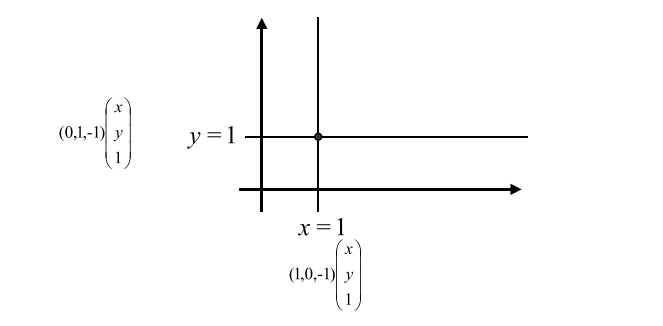
\includegraphics[width=0.8\columnwidth]{pictures/verticalhorizontal}

\textbf{Line joining two points}:
$$ \bm{l} = \bm{\tilde{x}_1} \times \bm{\tilde{x}_2} $$

\subsubsection{3D Planes}

$$ \pi = (\pi_1,\pi_2,\pi_3,\pi_4)^\top $$

The point $\bm{\tilde{X}}$ lies on the plane $\pi$ if and only if
$$ \pi^T\bm{\tilde{X}} = \pi_1x+\pi_2y+\pi_3z+\pi_4w = 0 $$

Planes from points
$$ \begin{bmatrix}
	\tilde{\bm{X}}^{(1)\top}\\
	\tilde{\bm{X}}^{(2)\top}\\
	\tilde{\bm{X}}^{(3)\top}\\
\end{bmatrix} \pi = 0 $$


\subsubsection{Conic}
Inhomogenious:
$$ ax^2 + bxy + cy^2 + dx + ey + f = 0$$

5 Degrees of freedom

\subsection{Transformation}
\subsubsection{2D Transformation}
\begin{itemize}
	\item Rotation+translation/Euclidean
	\item Scaled Rotation/Similarity/Metric - This transformation preserves angles between lines and planes( Orthogonal views of the planar at all times)
	\item Affine - Parallel lines and planes remain parallel under affine transformations (general camera motion relative to the planar shape, but always keeping sufficient distance from the planar shape)
	\item Projectivity/Collineation/Projective transformation/Homography (all cameras motions are allowed, also when moving close to the planar shape)
\end{itemize}

$$\begin{pmatrix}
x'\\
y'\\
w'\\
\end{pmatrix} = \begin{bmatrix}
h_{11}&h_{12}&h_{13}\\
h_{21}&h_{22}&h_{23}\\
h_{31}&h_{32}&h_{33}\\
\end{bmatrix} \begin{pmatrix}
x\\
y\\
w\\
\end{pmatrix} $$

Point transformation: $\bm{\tilde{x}'} = H \bm{\tilde{x}}$\\
Line transformation: $\bm{l'} = H^{-\top} \bm{l}$\\

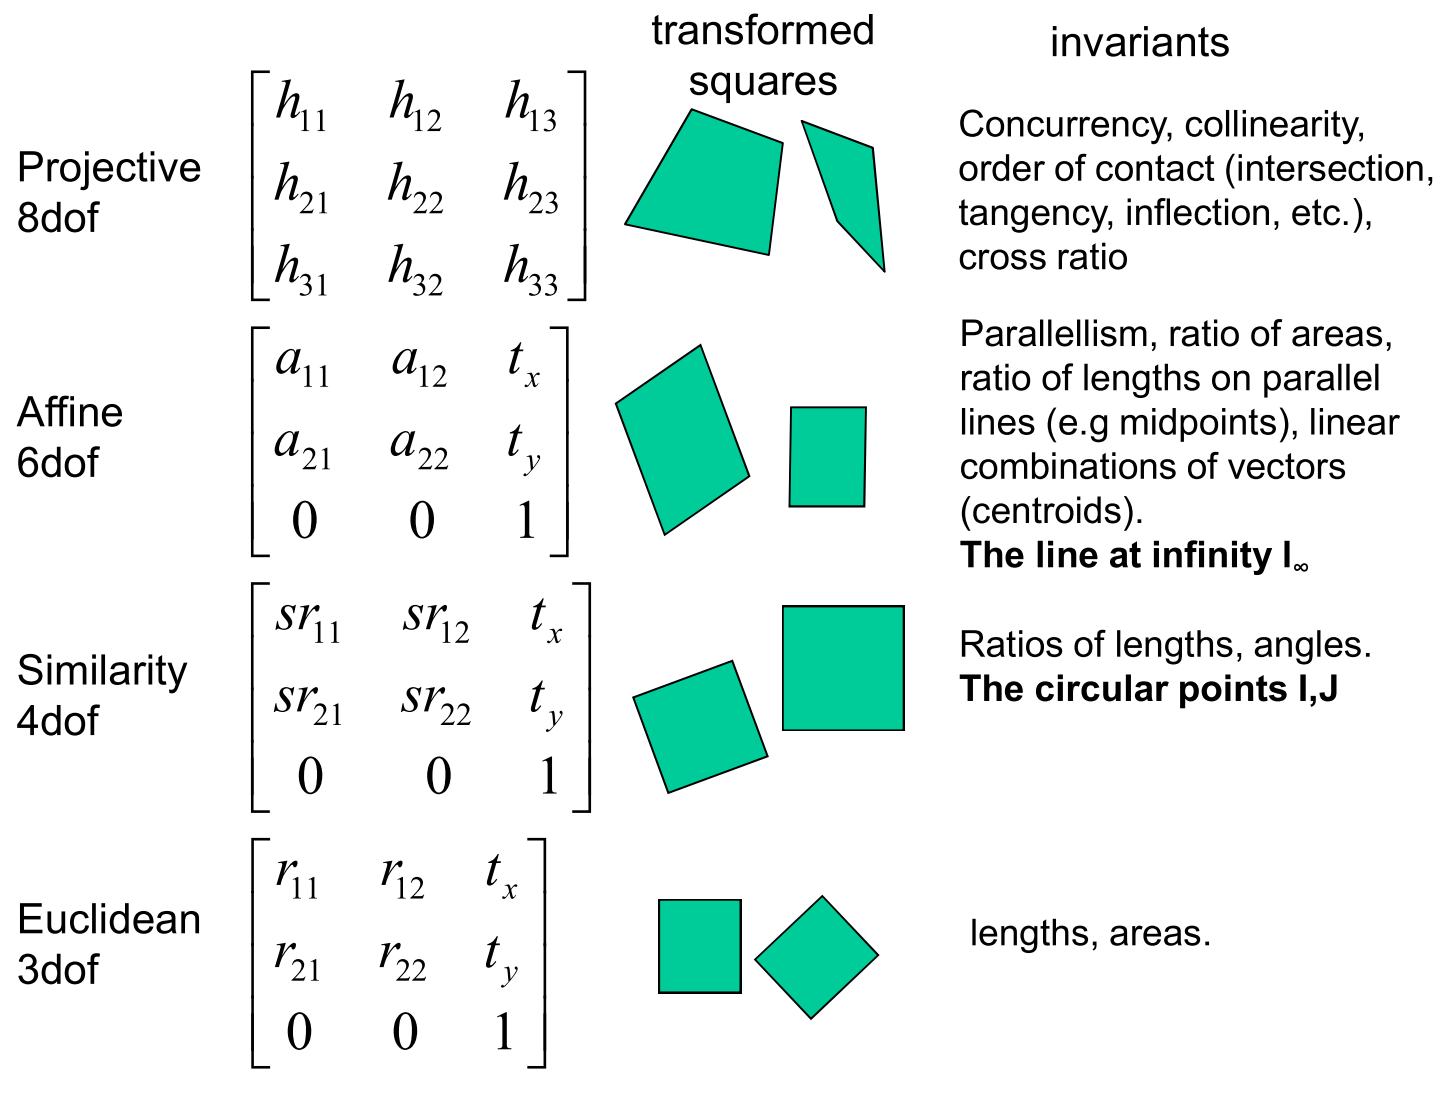
\includegraphics[width=\columnwidth]{pictures/2Dtransformations}

\subsubsection{3D Transformationen}

$$\begin{pmatrix}
x'\\
y'\\
z'\\
w'\\
\end{pmatrix} = \begin{bmatrix}
h_{11}&h_{12}&h_{13}&h_{14}\\
h_{21}&h_{22}&h_{23}&h_{24}\\
h_{31}&h_{32}&h_{33}&h_{34}\\
h_{41}&h_{42}&h_{43}&h_{44}\\
\end{bmatrix} \begin{pmatrix}
x\\
y\\
z\\
w\\
\end{pmatrix} $$

Point transformation: $\bm{\tilde{X}'} = H \bm{\tilde{X}}$\\
Plane transformation: $\bm{\pi'} = H^{-\top} \bm{\pi}$\\

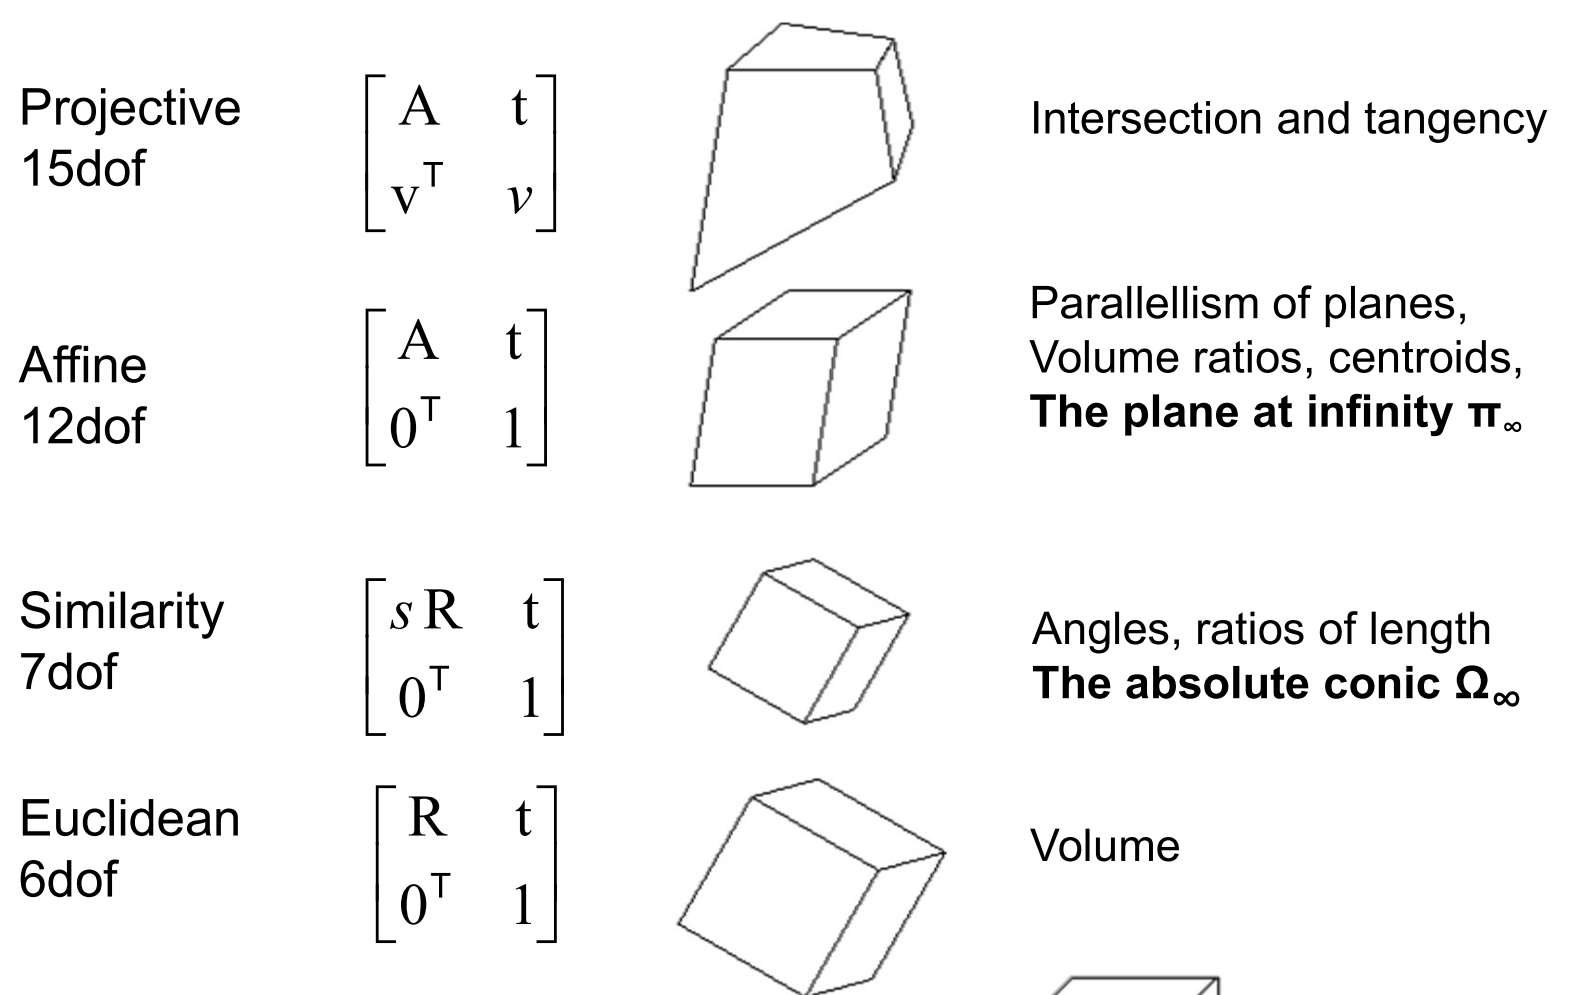
\includegraphics[width=\columnwidth]{pictures/3Dtransformation}


		%Chapter 1 - Mathe
	\section{Camera Model}
\subsection{Camera Matrix}
\subsubsection{Pinhole camera model}
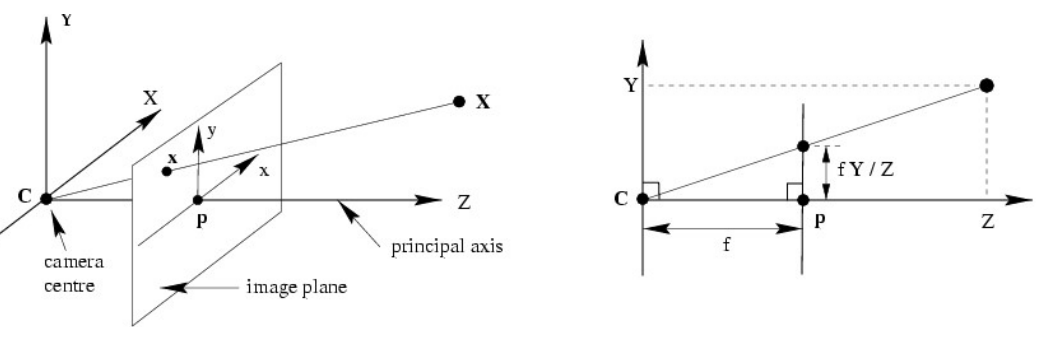
\includegraphics[width=\columnwidth]{pictures/pinholecamera}
Projection on image plane
$$\begin{pmatrix}
fX\\
fY\\
Z\\
\end{pmatrix} = 
\underbrace{\begin{bmatrix}
	f&0&0&0\\
	0&f&0&0\\
	0&0&1&0\\
	\end{bmatrix} }_{= diag(f,f,1)[I|0]} \begin{pmatrix}
X\\
Y\\
Z\\
1\\
\end{pmatrix} $$
By dividing $(fX,fY,Z)^\top$ by $Z$ we get $(x,y,1)^\top$

\subsubsection{Principal Point offset}
Moving the point into the middle of the picture

$$\begin{pmatrix}
fX+Zp_x\\
fY+Zp_y\\
Z\\
\end{pmatrix} = \begin{bmatrix}
f&0&p_x&0\\
0&f&p_y&0\\
0&0&1&0\\
\end{bmatrix} \begin{pmatrix}
X\\
Y\\
Z\\
1\\
\end{pmatrix} $$
By dividing $(fX+Zp_x,fY+Zp_y,Z)^\top$ by $Z$ we get $(x+p_x,y+p_y,1)^\top$

\subsubsection{Kalibration matrix K}
Intrinsic camera parameters

$$ \underbrace{K = \begin{bmatrix}
f&0&p_x\\
0&f&p_y\\
0&0&1\\
\end{bmatrix}}_{simple: a=1 \text{ and } s=0}  \qquad \underbrace{K = \begin{bmatrix}
f&s&p_x\\
0&af&p_y\\
0&0&1\\
\end{bmatrix}}_{general}$$

$f$: focal length\\
$s$: skew between the sensor axes due to the sensor not being mounted perpendicular to the optical axis\\
$a$: aspect ratio between $f_x$ \& $f_y$

\subsubsection{Camera Rotation + Shift}
Extrinsic camera parameters
$$ [R|t] $$
$R$: 3x3 Rotation matrix\\
$t$: 3x1 Translation vector

\subsubsection{Camera Matrix / Projective Camera}
$$ P = K[R|t] $$

$$ \lambda \begin{bmatrix}
u\\
v\\
1\\
\end{bmatrix} = P \begin{bmatrix}
X\\
Y\\
Z\\
W\\
\end{bmatrix} = K[R|t] \begin{bmatrix}
X\\
Y\\
Z\\
W\\
\end{bmatrix} $$

Full matrix has 11 DOF (5 intrinsic +3 rot +3 trans)

3x4 matrix

$$ \tilde{P} = \begin{bmatrix}
K&0\\
0&1\\
\end{bmatrix} \begin{bmatrix}
R&t\\
0^T&1\\
\end{bmatrix} $$
4x4 matrix

$$P = K[R|-RC]$$

\subsection{Camera Calibration with Direct Linear Transform (DLT)}
The DLT method uses a set  of  control  points  whose  object  space/plane  coordinates  are  already  known.  The  control  points  are  normally  fixed  to  a  rigid  frame,  known  as  the  calibration  frame.    The  problem  is  essentially  to  calculate  the  mapping  between  the  2D  image  space  coordinates  (x,y)  and  the  3D  object  space  coordinates  (X,Y,Z).  For this 3D $\leftrightarrow$ 2D correspondence the mapping should take the form of a 3x4 projection matrix (P) such that $x = PX$.

$$ x = PX \rightarrow [x]_xPX = 0 $$

Denoting the rows of $P$ with $P^1, P^2, P^3$ we can rewrite above equation to

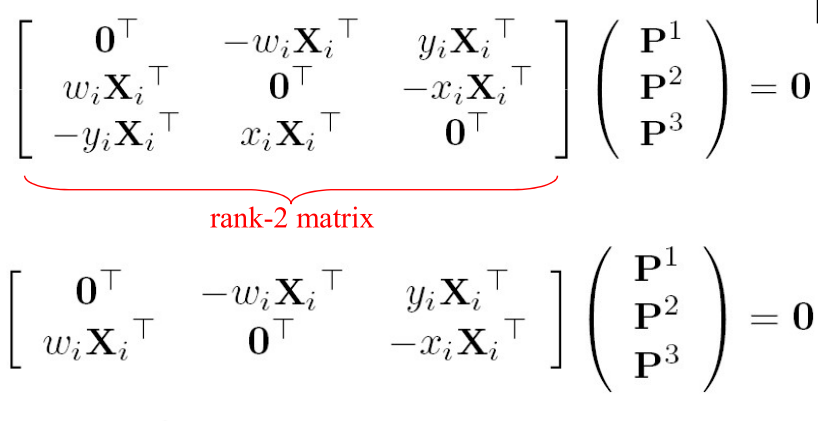
\includegraphics[width=0.7\columnwidth]{pictures/dlt}

Since the third equation is dependant on the first two, it can be discounted. So for every point X we get two equations.

The bracket is denoted with $A$ (2nx12) and the camera matrix with P (3x4)
  
$$ A P = 0 $$

P has 11 DOF $\rightarrow$ 5.5 points are needed for the minimal solution.
For $n \geq 6$ it is over-determined and is solved with SVD.

\subsubsection{Gold Standard algorithm}
Objective:\\
Given $n \geq 6$ 2D to 3D point correspondences, determine the Maximum Likelihood Estimation of the camera projection matrix P.\\

Algorithm:
\begin{enumerate}
	\item Linear Solution: Compute an initial estimate of P using a linear method.
		\begin{enumerate}
			\item Normalization $\tilde{X} = UX$, $\tilde{x} = Tx$
			\item DLT
		\end{enumerate}
	\item Minimization of geometric error: using the linear estimate as a starting point minimize the geometric error: $\min_P \sum_{i}d(\tilde{x}_i,\tilde{P}\tilde{X}_i)^2$
	\item Denormalization $P = T^{-1}\tilde{P}U$
\end{enumerate} 			%Chapter 2 - Kalibration
	\section{Feature Matching}
Feature: measured characteristic of (part of) a pattern / object\\
Goal: efficient matching


Features shoud overcome large variations in
\begin{enumerate}
	\item Viewpoint
	\item Illumination
	\item Background
	\item Occlusions
	\item Scale change
	\item Deformation
	\item Perspective Deformation
	\item Blur
\end{enumerate}

A feature should capture something \textbf{discriminative} about a well \textbf{localisable} patch of a surface

\subsection{Detector}

The detector typically yields image points. Corners are the most prominent example of so-called `Interest Points’, i.e. points that can be well localised in different views of a scene

\subsubsection{Uniqueness of a patch}
How do the patterns change upon a shift?\\
\textit{flat region}: no change in all directions\\
\textit{edge region}: no change along edge direction\\
\textit{corner} : significant change in all directions\\
\\
Compare each pixel before and after by summing up the squared differences (SSD) - this defines an error $E(u,v)$. Shift in x-direction: $u$, in y-direction:$y$.
$$ E(u,v) = \sum_{(x,y)\in W} [I(x+u, y+v) - I(x,y)]^2 $$
$$ E(u,v) = \sum_{(x,y)\in W} [u v] \underbrace{\begin{bmatrix}
I_x^2&I_xI_y\\
I_yI_x&I_y^2\\
\end{bmatrix}}_H \begin{bmatrix}
u\\
v\\
\end{bmatrix} $$
Want E(u,v) to be \textbf{large} for small shifts in \textbf{all} directions - the minimum is given by the smaller eigenvalue of H.

\subsubsection{The Harris corner detector}
$$ R = det(H) - k*trace(H)^2 $$
When $|R|$ is small, which happens when $\lambda_1$ and $\lambda_2$ are small, the region is flat.\\
When $R<0$, which happens when $\lambda_1$>>$\lambda_2$ or vice versa, the region is an edge.\\
When $|R|$ is large, which happens when $\lambda_1$ and $\lambda_2$ are large and $\lambda_1 ~\lambda_2$, the region is a corner.

\subsection{Descriptor}
Descriptors then are a vector of measurements taken around each such point


We need to describe their surrounding image patch such we can discriminate between them, i.e. we need to build a feature vector for the patch \&
Invariance under geom./phot. change

\subsubsection{Deformations under projections (geom. change)}
\begin{enumerate}
	\item similarity 4DOF
	\item affinity 6DOF
	\item projectivity 8DOF
\end{enumerate}

Complexity of the groups goes up with the generality of the viewing conditions, and so does the complexity of the group’s invariants. Fewer invariants are found going from top to bottom

\subsubsection{Photometric changes}
\begin{itemize}
	\item Contrasts (intensity differences) let the non-linear offsets cancel; hence gradients are good !
	\item Moreover the orientation of gradients in the color bands is invariant under their linear changes, as is the intensity gradient orientation in case the scale factors are identical; this is indeed relevant if the illumination changes its intensity, but not its color, which is typically assumed.
	\item But even under changing color of the illumination, in practice edge orientations tend to remain the same.
\end{itemize}

\subsection{Matching}
\begin{itemize}
	\item Interest points are matched on the basis of their descriptors
	\item E.g. nearest neighbour, based on some distance like Euclidean or Mahalanobis; good to compare against 2nd nearest neighbour: OK if difference is big; or fuzzy matching w. multiple neighbours
	\item Speed-ups by using lower-dim. descriptor space (PCA) or through some coarse-to-fine scheme (very fast schemes exist to date!)
	\item Matching of individual points typically followed by some consistency check, e.g. epipolar geometry, homograpy, or topological
\end{itemize}

\subsection{The Patch}
\subsubsection{MSER - Maximally stable extremal regions}
\begin{enumerate}
	\item Start with intensity extremum
	\item Then move intensity threshold away from its value and watch the super/sub-threshold region grow
	\item Take regions at thresholds where the growth is slowest (happens when region is bounded by strong edges)
\end{enumerate}

\subsubsection{SIFT - Scale-Invariant Feature Transform}
Is a carefully crafted interest point detector + descriptor, based on intensity gradients and invariants under similarities, not affine like so far.\\
\\
\textbf{Descriptor} is based on blob detection - at several scales - that is local extrema of the Laplacian-of-Gaussian (LoG)

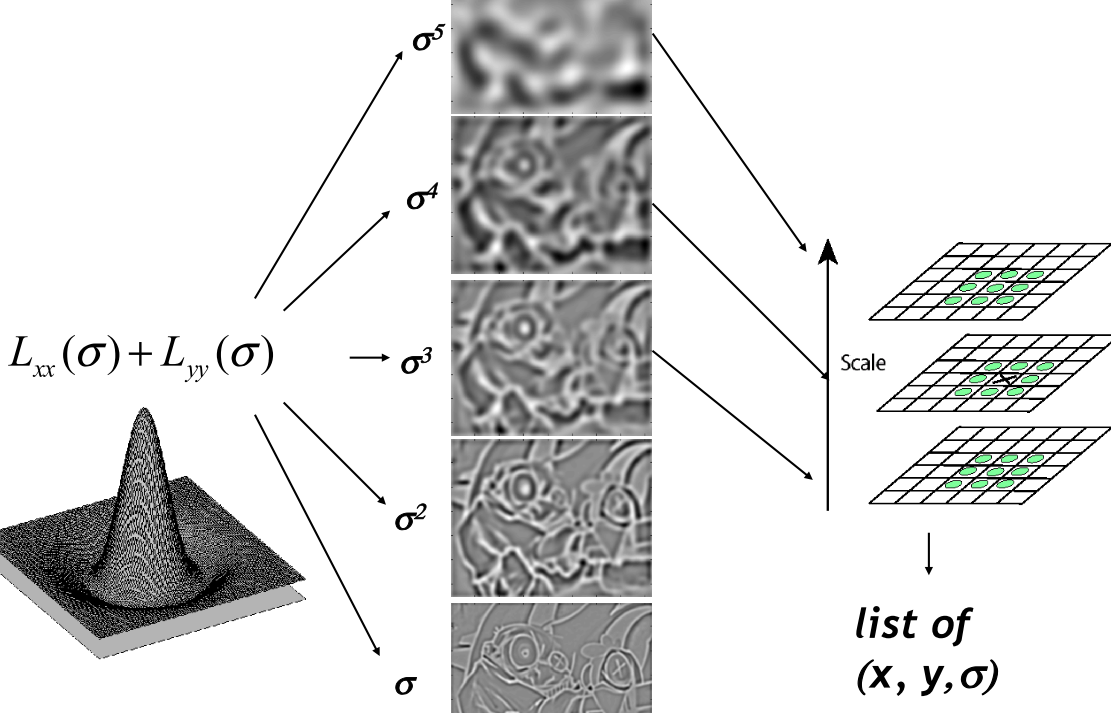
\includegraphics[width=0.7\columnwidth]{pictures/sift2}

\begin{itemize}
	\item Thresholded image gradients are sampled over a grid - Dominant orientation selection
	\begin{itemize}
		\item Compute image gradients of cell
		\item Build orientation histogram
		\item Find maximum of cell $\rightarrow$ orientation of cell
	\end{itemize}
	\item Create array of orientation histograms within blocks
	\item 8 orientations x 4x4 histogram array (! in picture only 2x2) = 128 dimensions
	\item Apply weighting with a Gaussian located at the center
	\item Normalized to unit vector
\end{itemize}

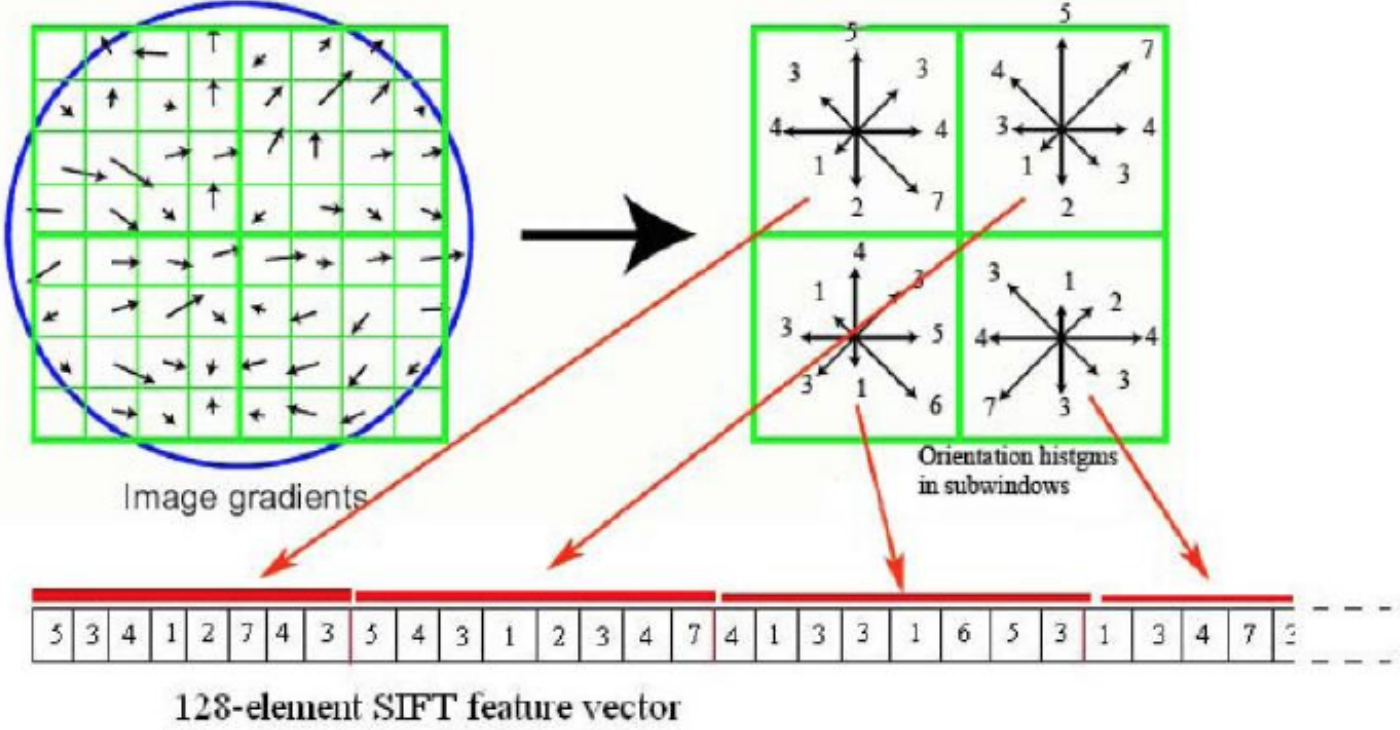
\includegraphics[width=\columnwidth]{pictures/sift}

\subsubsection{SURF - efficient alternative to SIFT}
no further infos			%Chapter 3 - Feature extraction
	\section{Motion Extraction}
Motion can be the only cue for segmentation - camouflage is only visible in motion\\
\\
Some applications of motion extraction:
\begin{itemize}
	\item change / shot cut detection in films
	\item surveillance / traffic monitoring
	\item autonomous driving
	\item analyzing game dynamics in sports
	\item motion capture / gesture analysis
	\item image stabilisation
	\item motion compensation (e.g. medical robotics)
	\item feature tracking for 3D reconstruction (structure from motion)
\end{itemize}

\subsection{Optical Flow}
Optical Flow = apparent motion of brightness patterns\\
\\
Ideally, the optical flow is the projection of the threedimensional motion vectors on the image - Such 2D motion vector is sought at \textbf{every} pixel of the image (a motion vector here is a 2D translation vector)\\
\\
Suppose a point of the scene projects to a certain pixel of the current video frame. Our task is to figure out to which pixel in the next frame it moves…
In order to find these corresponding pixels, we need to come up with a reasonable assumption on how we can detect them among the many.
We assume these corresponding pixels have the same intensities as the pixels the scene points came from in the previous frame.\\
\\
Two examples where following brightness patterns is misleading:
\begin{enumerate}
	\item Untextured, rotating sphere $O.F. = 0$
	\item No motion, but changing lighting $O.F. \neq 0$
\end{enumerate}

\subsubsection{Mathematical formulation}
I (x,y,t) = brightness at (x,y) at time t - one equatio per pixel

$$
\frac{DI}{Dt} = \frac{\partial I}{\partial x}\frac{\partial x}{\partial t}+\frac{\partial I}{\partial y}\frac{\partial y}{\partial t}+\frac{\partial I}{\partial t} = I_x u + I_y v + I_t = 0
$$

The three derivates can be measured but the velocity u,v are unknown.

\textit{something calculus}



Horn \& Schunck algorithm

\textit{something solution of problem}

\begin{itemize}
	\item errors at object boundaries
	\item example of regularization
\end{itemize}

\subsection{Condensation Filter {\small or condensation tracker}}

System model (f = system transition function)
$$x_t = f_{t-1}(x_{t-1},w_{t-1}) $$
Measurement model (h = measurement function)
$$ z_t = h_t(x_t,v_t) $$
and $Z_t = (z_1, \dots , z_t)$ is the history of observations\\

\subsubsection{Recursive Bayesian filter (Kalman filter)}
Object not as a single state but a probabilistic distribution.\\
\\
1. prediction
$$
p(x_t | Z_{t-1}) = \int p(x_t | x_{t-1}) p(x_{t-1} | Z_{t-1}) dx_{t-1}
$$
2. measurement update
$$
p(x_t | Z_t) = \frac{p(Z_t | x_t) p(x_t | Z_{t-1})}{p(Z_t | Z_{t-1})}
$$

Problem integral is computational heavy to compute -> condensation tracker (particle filter)

\subsubsection{Particle Filter}
\begin{multicols}{2}
	1. prediction\\
	Start with $S_{t-1}$, the sample set of the previous step, and apply the system model to each sample, yielding predicted samples $s_t$.\\
	2. update\\
	Scale each particle by the measurement likelihood. Weight the particles.\\
	3. resample\\
	resample to get $N$ particles with equal weights.
	
	\columnbreak
	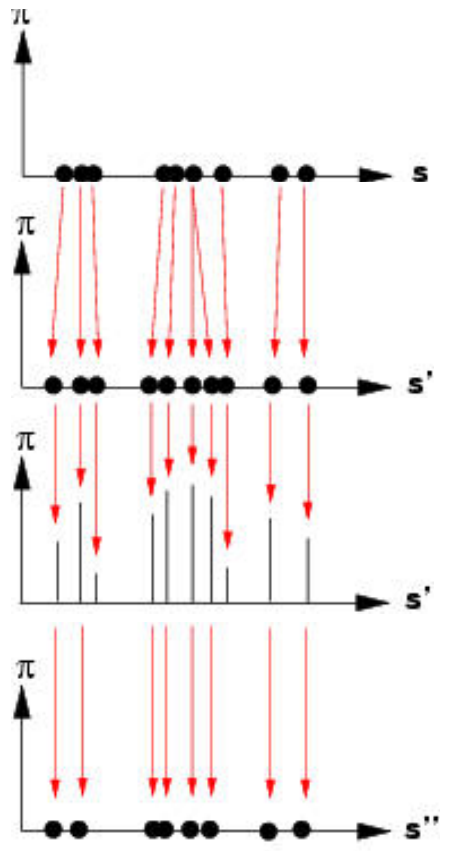
\includegraphics[width=0.7\columnwidth]{pictures/particlefilter}
\end{multicols}

In the limit (large N) equivalent to Bayesian tracker

\subsubsection{Comparison Particle Filter - Kalman filter}
{\footnotesize \begin{multicols}{2}
	\begin{itemize}
		\item Unrestricted system models
		\item Unrestricted noise models
		\item Multiple hypotheses
		\item Discretisation error
		\item Postprocessing for interpret
	\end{itemize}
	\columnbreak
	\begin{itemize}
		\item Linear system models
		\item Gaussian noise
		\item Unimodal
		\item Exact solution
		\item Direct interpretation
	\end{itemize}
\end{multicols}}
		%Chapter 4 - Structure and Motion
	\section{Multiple View Geometry}

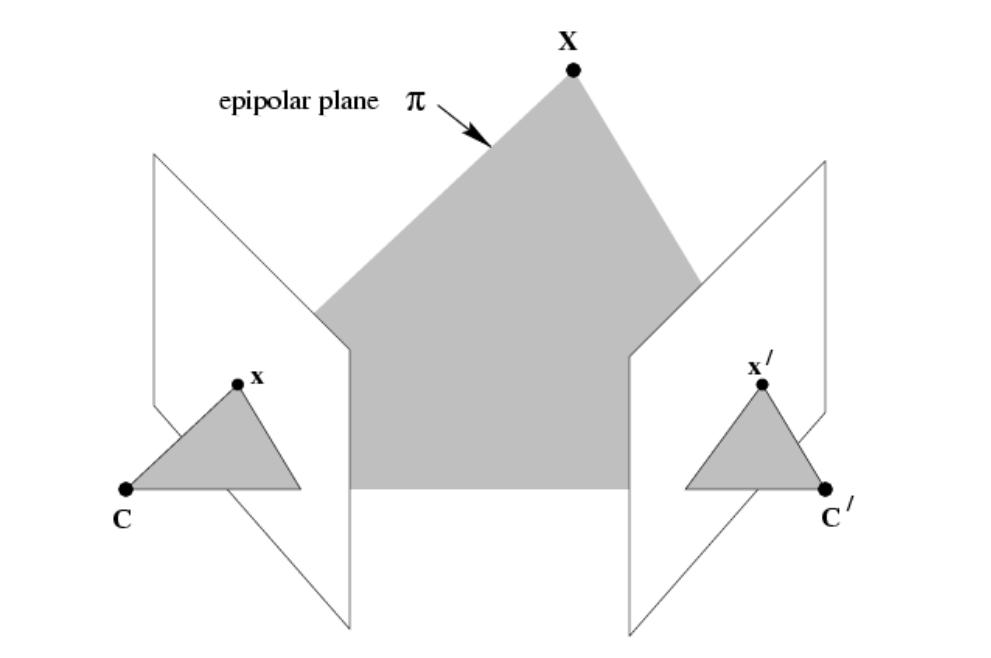
\includegraphics[width=\columnwidth]{pictures/epipolarplane}

All points on $\pi$ project on l and l’

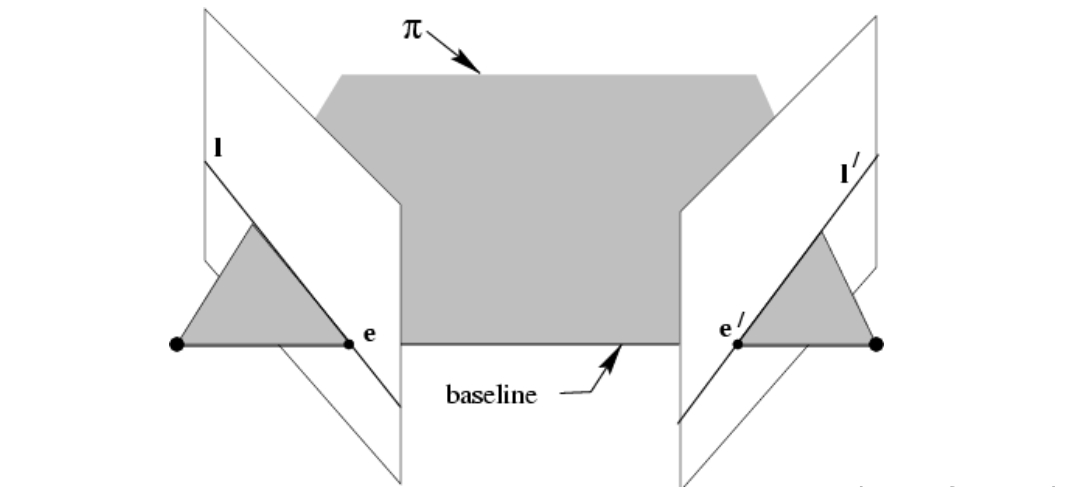
\includegraphics[width=\columnwidth]{pictures/epipolarplane2}

epipoles e,e’
\begin{itemize}
	\item intersection of baseline with image plane
	\item projection of projection center in other image
	\item vanishing point of camera motion direction\\
	\end{itemize}

an epipolar plane ($\pi$)
\begin{itemize}
	\item plane containing baseline (1-D family)\\
\end{itemize}

an epipolar line ($l$) 
\begin{itemize}
	\item intersection of epipolar plane with image (always come in corresponding pairs)\\
\end{itemize}

epipolar lines from motion

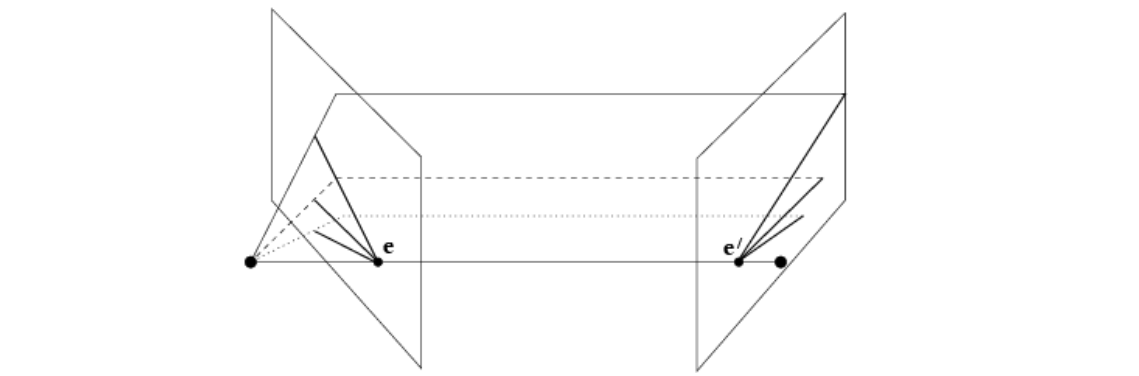
\includegraphics[width=0.8\columnwidth]{pictures/motion}

parallel motion

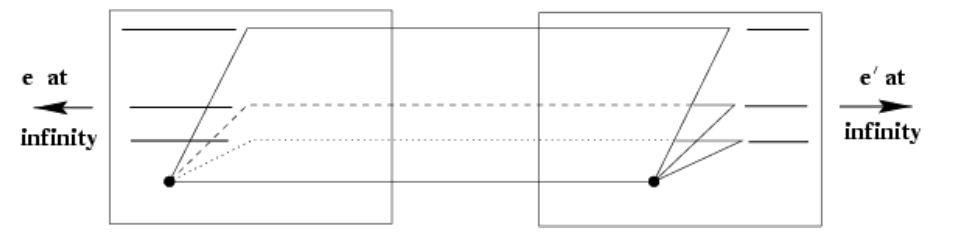
\includegraphics[width=0.8\columnwidth]{pictures/parallelmotion}

forward motion

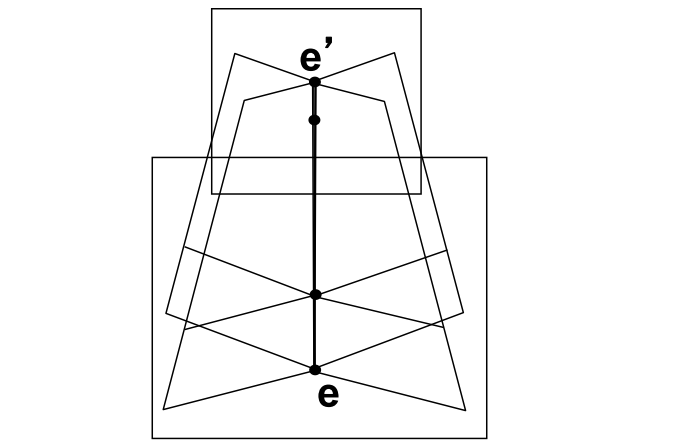
\includegraphics[width=0.4\columnwidth]{pictures/forwardmotion}

\subsection{Fundamental matrix}

$$l' = e' \times x' = e' \times Hx = Fx$$

The fundamental matrix F is independent of the point.

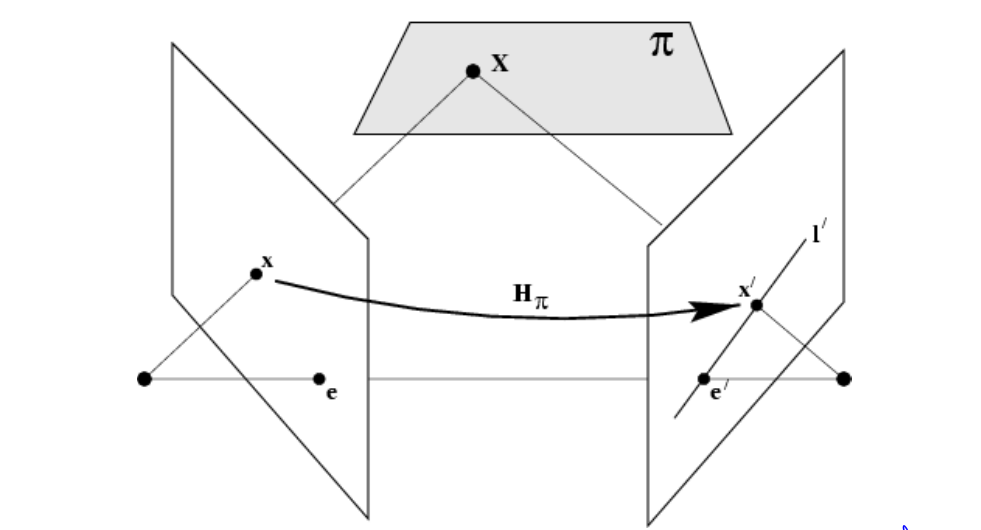
\includegraphics[width=\columnwidth]{pictures/epipolarplane3}

correspondence condition: 
$$x'^TFx=x'^T l'=0$$

\begin{itemize}
	\item transpose: if F is fundamental matrix for (P,P'), then transp(F) is fundamental matrix for (P',P)
	\item Epipolar lines: l'=Fx and l=transp(F)x'
	\item Epipoles: on all epipolar lines, thus transp(e')Fx=0 for all x therefore transp(e')F = 0, similarly Fe=0
	\item F has 7 DOF i.e. 3x3-1(homogeneous)-1(rank2)
	\item F is a correlation, projective mapping from a point x to a line l'=Fx (not a proper correlation, i.e. not invertible)
\end{itemize}

for pure translation F only has 2 degrees of freedom

\subsubsection{Eight-Point Algorithm}
Since the fundamental matrix F is a 3x3 matrix determined up to an arbitrary scale factor, 8 linear equations are required to obtain a unique solution. It is possible with 7.

\subsection{Essential Matrix}
for the calibrated case

5 linear equations are needed.

Same as Fundamental matrix
\begin{itemize}
	\item Ep' is the epipolar line associated with p'
	\item transp(E)p is the epipolar line associated with p
	\item Ee'=0 and transp(E)e=0
	\item E is singular
\end{itemize}

New

\begin{itemize}
	\item E has two equal non-zero singular values
\end{itemize}


\subsection{Multi-view geometry}


\subsection{Dealing with Wide FOV Camera}
\begin{itemize}
	\item Two-step linear approach to compute radial distortion
	\item estimates distortion polynomial of arbitrary degree
\end{itemize}	%Chapter 5 - Multiple View Geometry
	\section{Model fitting}

\subsection{Hough transform}

x-y space to a-b parameter space

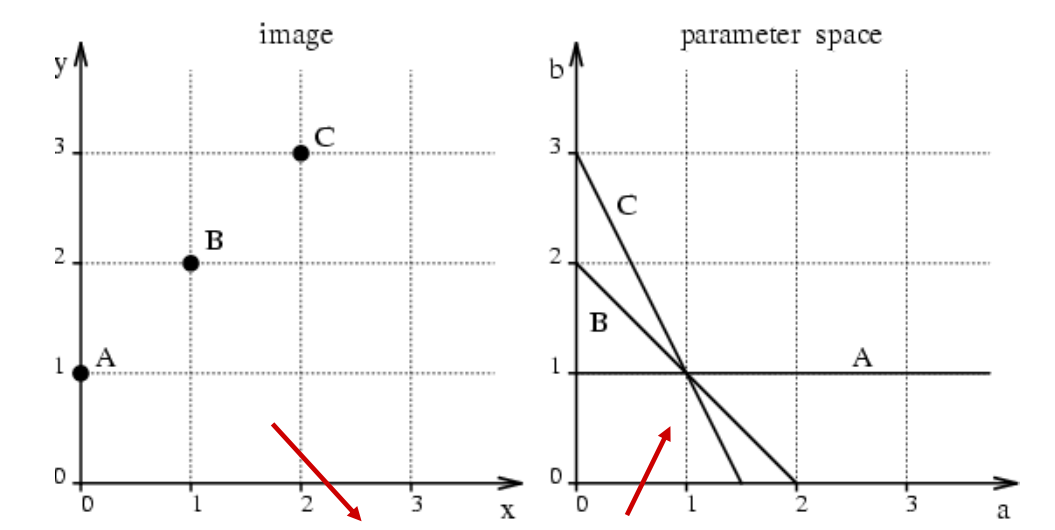
\includegraphics[width=0.8\columnwidth]{pictures/hough}

$$b = (-x)*a+y$$

Alternative: x-y space to $\theta$-$\rho$ (or d) space
$$x cos(\theta) + y sin(\theta) = \rho$$

For each point, render the curve ($\theta$, d) and count the parameter in bins with similar values.

Difficulties: How big should the bins be (too big, and we cannot distinguish between quite different lines; too small, and noise causes lines to be missed)


Hardly ever satisfactory in practice, because problems with noise and bin size defeat it

\subsection{Line fitting}
\subsubsection{Incremental line fitting}
\begin{lstlisting}[frame=single]
Put all points on a curve list, in order along the curve
Empty the line point list
Empty the line list
Until there are too few points on the curve
	Transfer first few points on the curve tot the line point list
	Fit line to line point list
	While fitted line is good enough
		Transfer the next point on the curve to tthe line point list and refit the line
	end
	Transfer last point(s) back to curve
	Refit line
	Attach line to line list
end
\end{lstlisting}  

\subsubsection{K-means}
\begin{lstlisting}[frame=single]
Hypothesize k lines (perhabps uniformly at random)
or
Hypothesize an assignment of lines to points and then fit lines using this assingment

Until convergence
	Allocate each point to the closest line
	Refit lines
end
\end{lstlisting} 

Problem can be stuck in local optima
 
\subsubsection{Probabilistic}
- EM-algorithm (expectation maximum)
- M-estimators
- RANSAC

\subsubsection{RANSAC}

- Choose a small subset uniformly at random
- Fit to that
- Anything that is close to result is signal; all others are noise
- Refit
- Do this many times and choose the best\\

\textbf{Issues} 
\begin{itemize}
	\item How many times? Often enough that we are likely to have a good line
	\item How big a subset? Smallest possible
	\item What does close mean? Depends on the problem
	\item What is a good line? One where the number of nearby points is so big it is unlikely to be all outliers
\end{itemize}


\begin{lstlisting}[frame=single]
Determine:
	n-the smallest number of points required
	k-the number of iterations required
	t-the threshold used to identify a point that fits well
	d-the number of nearby points required to assert a model fits well
Until k iterations have occured
	Draw a sample of n points from the data uniformly and at random
	Fit to that set of n points
	For each data point outside the sample
		Test the distance from the point to the line against t; if the distance from the point to the line is less than t, the point is close
	end
	If there are d or more points close to the line then there is a good fit. Refit the line using all these points.
end
Use the best fit from this collection, using the fitting error as criterium	
\end{lstlisting} 

$$ k = \frac{log(1-p)}{log(1-w^s)} $$
k - number of iterations\\
p - probability at least one sample free from outliers\\
w - fraction of inliers = d/n\\
s - model dimension (2 for a line, 3 for plane)

\subsection{Missing variable problems}

In many vision problems, if some variables were known the maximum likelihood inference problem would be easy 
\begin{itemize}
	\item fitting; if we knew which line each token came from, it would be easy to determine line parameters
	\item segmentation; if we knew the segment each pixel came from, it would be easy to determine the segment parameters
	\item fundamental matrix estimation; if we knew which feature corresponded to which, it would be easy to determine the fundamental matrix
\end{itemize}
This sort of thing happens in statistics, too - strategy:
\begin{enumerate}
	\item estimate missing variables
	\item plug these in, now estimate parameters
	\item re-estimate appropriate values for missing variables - converges to local extremum (like k-means)
\end{enumerate}

\subsection{Cross validation}
-Split data set into two pieces, fit to one, and compute negative loglikelihood on the other
-Average over multiple different splits
-Choose the model with the smallest value of this average
-The difference in averages for two different models is an estimate of the difference in KL divergence of the models from the source of the data			%Chapter 6 - Model Fitting
	\section{Image segmentation}
Identify groups of pixels that belong together - goal: Delineate objects and background regions \& group similar-looking pixels for efficientcy of further processing

Examples of Groupin in vision
\begin{itemize}
	\item similar appearance
	\item symmetry
	\item common fate (direction etc)
	\item proximity
\end{itemize}

\subsection{Segmentation as clustering}
\subsubsection{Clustering}
Chicken and Egg problem  - either know the centers and allocate the points to it OR know the point membership and create center from them

Feature space - depending on that choice we can group pixels in different ways

\begin{itemize}
	\item pixel intensity
	\item pixel color
	\item pixel texture
	\item pixel intensity + position (proximity)
\end{itemize}

\subsubsection{k-Means}
Idea: randomly initialize the k cluster centers, and iterate between the two steps from clustering

Properties: will always converge to some solution (which can be a local maximum)

Pro:
\begin{itemize}
	\item simple, fast to compute
	\item converges (to local maximum)
\end{itemize}

Cons:
\begin{itemize}
	\item number of cluster has to be defined
	\item sensitive to initial centers
	\item sensitive to outliers
	\item detects spherical clusters only
	\item assuming means can be computed
\end{itemize}
\subsubsection{Mixture of Gaussians, EM}
Idea: instead of treating the data as a bunch of points, assume that they are all generated by sampling a continous function - this function is called a \textit{generative model}, defined by a vector of parameters $\theta$

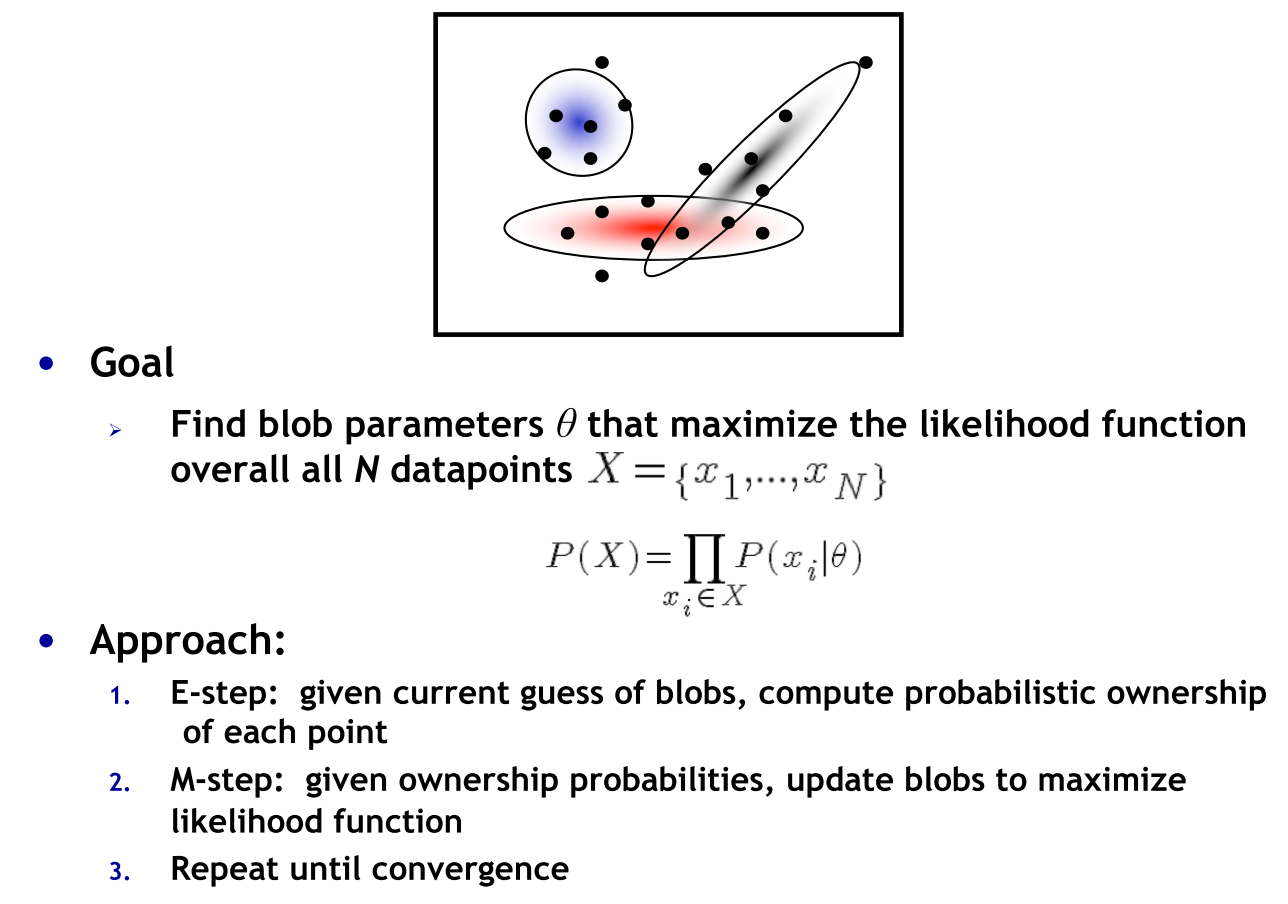
\includegraphics[width=\columnwidth]{pictures/EM}

E-Step: Compute probability that point $x$ is in blob b, given current guess of $\theta$

$$ P(b|x,\mu_b, V_b) = \frac{\alpha_b P(x|\mu_b, V_b)}{\sum_{i=1}^{K}\alpha_i P(x|\mu_i, V_i)} $$

M-Step: Compute overall probability that blob b is selected (N: data points)\\

Weight:
$$\alpha_b^{new} = \frac{1}{N} \sum_{i=1}^{N} P(b|x_i, \mu_b, V_b) $$
Mean of blob b:
$$ \mu_b^{new} = \frac{\sum_{i=1}^{N} x_i P(b|x_i, \mu_b, V_b)}{\sum_{i=1}^{N} P(b|x_i, \mu_b, V_b)}$$
Covariance of blob b:
$$ V_b^{new} = \frac{\sum_{i=1}^{N} (x_i-\mu_b^{new})(x_i-\mu_b^{new})^T P(b|x_i, \mu_b, V_b)}{\sum_{i=1}^{N} x_i P(b|x_i, \mu_b, V_b)} $$

EM Application is useful for all sorts of problems 
\begin{itemize}
	\item Any clustering problem
	\item Many model estimation problems
	\item Missing data problems
	\item Finding outliers
	\item Segmentation problems
	\begin{itemize}
		\item based on color
		\item based on motion
		\item Foreground/background separation 
\end{itemize}	
\end{itemize}
Pro:
\begin{itemize}
	\item Probabilistic interpretation
	\item Soft assignments between data points and clusters
	\item Generative model, can predict novel data points 
	\item Relatively compact storage ($O(Kd^2$)
\end{itemize}
Cons:
\begin{itemize}
	\item Initialization – often a good idea to start from output of k-means
	\item Local minima
	\item Need to know number of components K – Solutions: model selection (AIC, BIC), Dirichlet process mixture
	\item  Need to choose blob generative model (math form of a cluster?)
	\item Numerical problems are often a nuisance
\end{itemize}

\subsubsection{Mean-Shift Algorithm}
Choose features (color, gradients, texture, etc)
\begin{enumerate}
	\item Initialize random seed center and window size $W$
	\item Calculate center of gravity (the “mean”) of $W$: $ \sum_{x \in W} x H(x) $
	\item Shift the search window to the mean
	\item Repeat steps 2+3 until convergence for all centers
	\item merge windows that end up near the same peak/center
\end{enumerate}

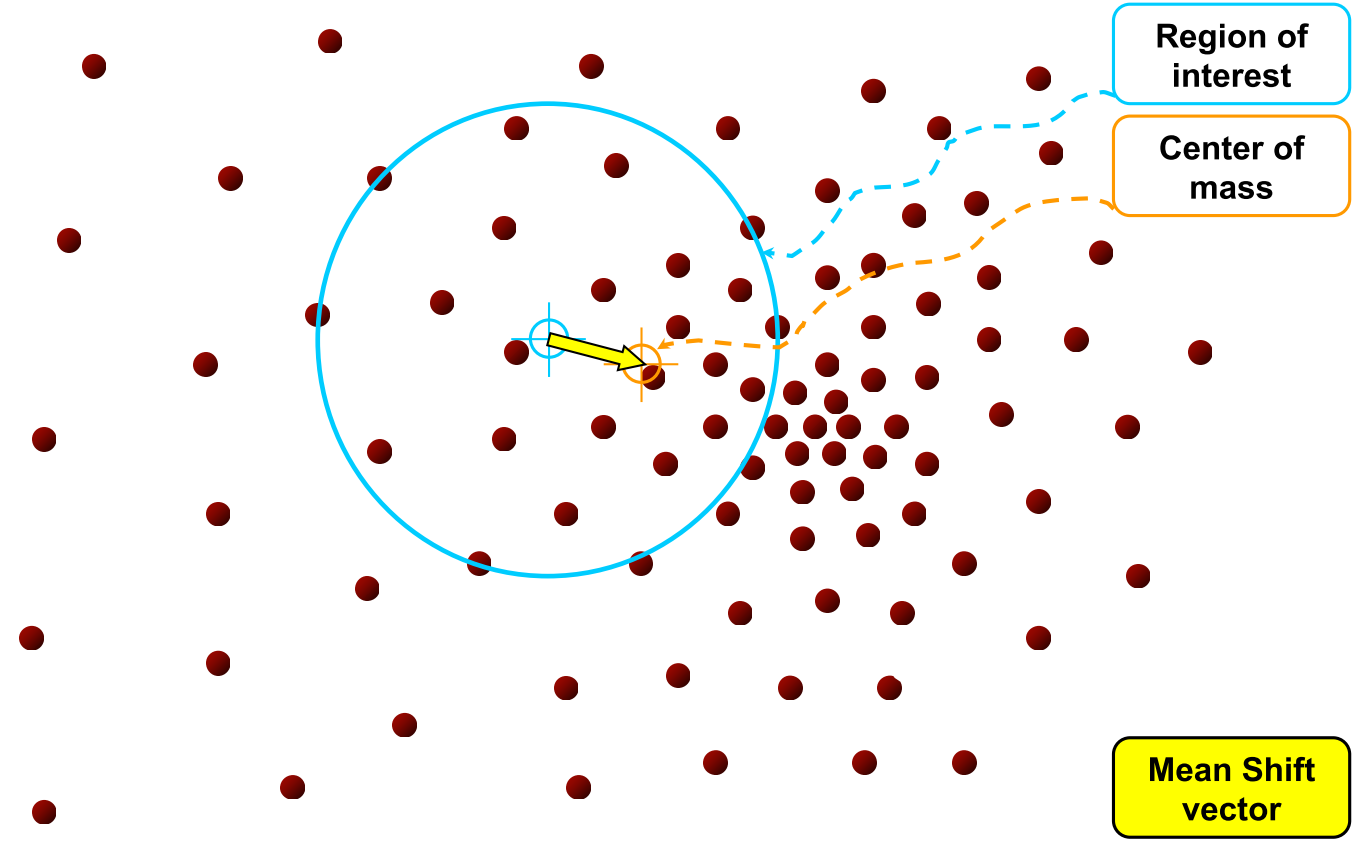
\includegraphics[width=\columnwidth]{pictures/meanshift}

Pro:
\begin{itemize}
	\item General, application-independent tool
	\item Model-free, does not assume any prior shape (spherical, elliptical, etc.) on data clusters
	\item Just a single parameter (window size h) – h has a physical meaning (unlike k-means) == scale of clustering
	\item Finds variable number of modes given the same h 
	\item Robust to outliers
\end{itemize}
Cons:
\begin{itemize}
	\item Output depends on window size h
	\item Window size (bandwidth) selection is not trivial
	\item Computationally rather expensive
	\item Does not scale well with dimension of feature space
\end{itemize}

\subsection{Hough transform}
see chapter before

\subsection{Interactive Segmentation with GraphCuts}
Markov Random Fields

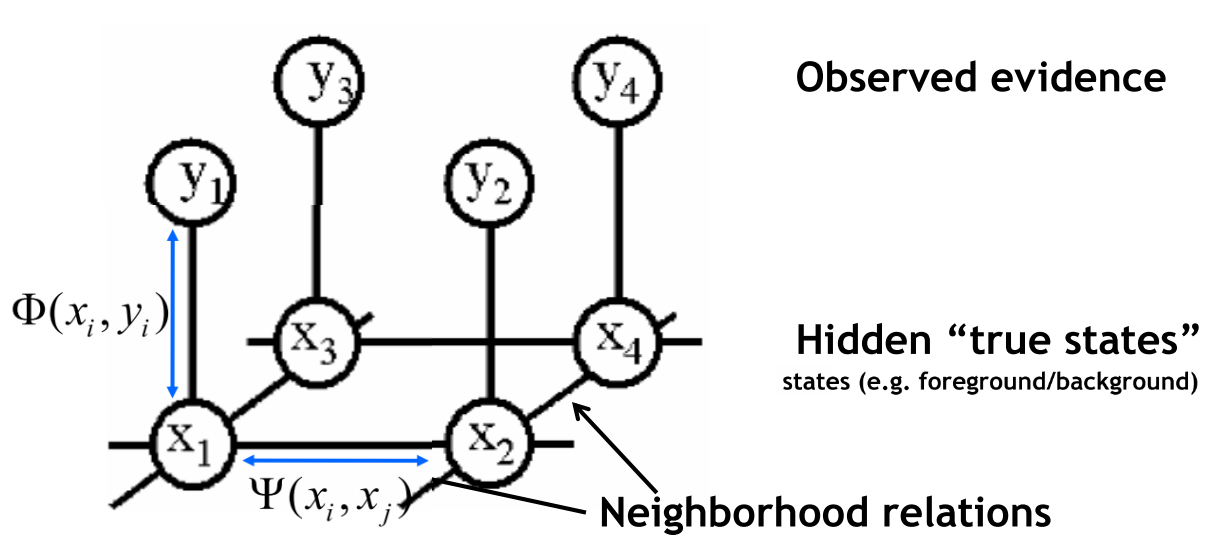
\includegraphics[width=\columnwidth]{pictures/markovfields}

Field Joint Probability

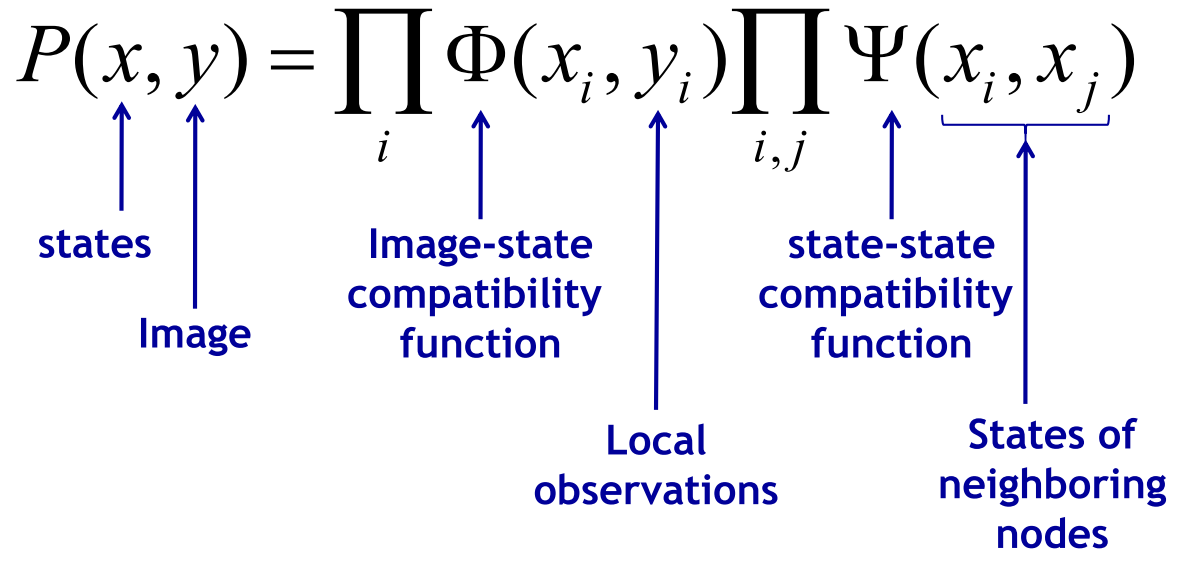
\includegraphics[width=0.7\columnwidth]{pictures/fieldjointprobability}

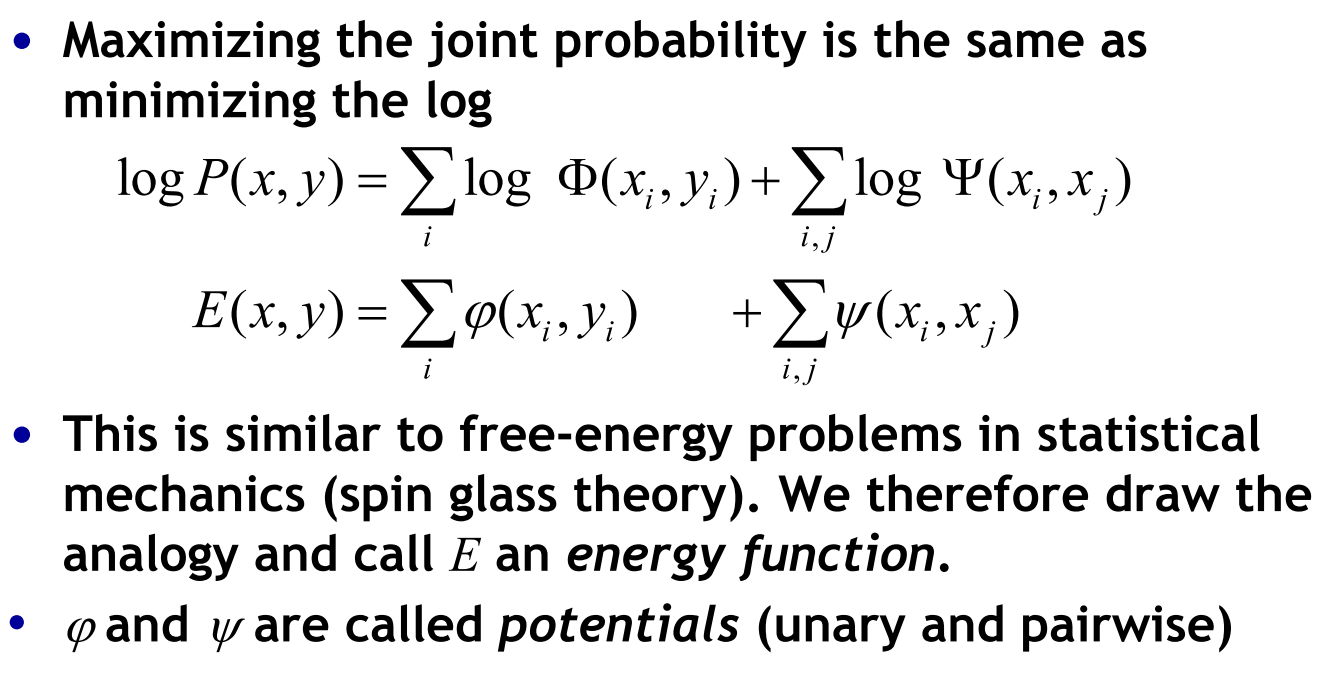
\includegraphics[width=\columnwidth]{pictures/energyfunction}
Unary potentials $\Phi$
\begin{itemize}
	\item Encode local information about the given pixel/patch
	\item How likely is a pixel/patch to be in a certain state (e.g. foreground/background)
\end{itemize}
Pairwise potentials $\Psi$
\begin{itemize}
	\item Ecode neighborhood information
	\item How different is a pixel/patch's label from that of its neighbor (e.g. here independent of image data, but later based on intensity/color/texture difference)
\end{itemize}

Goal: minimum cost cut

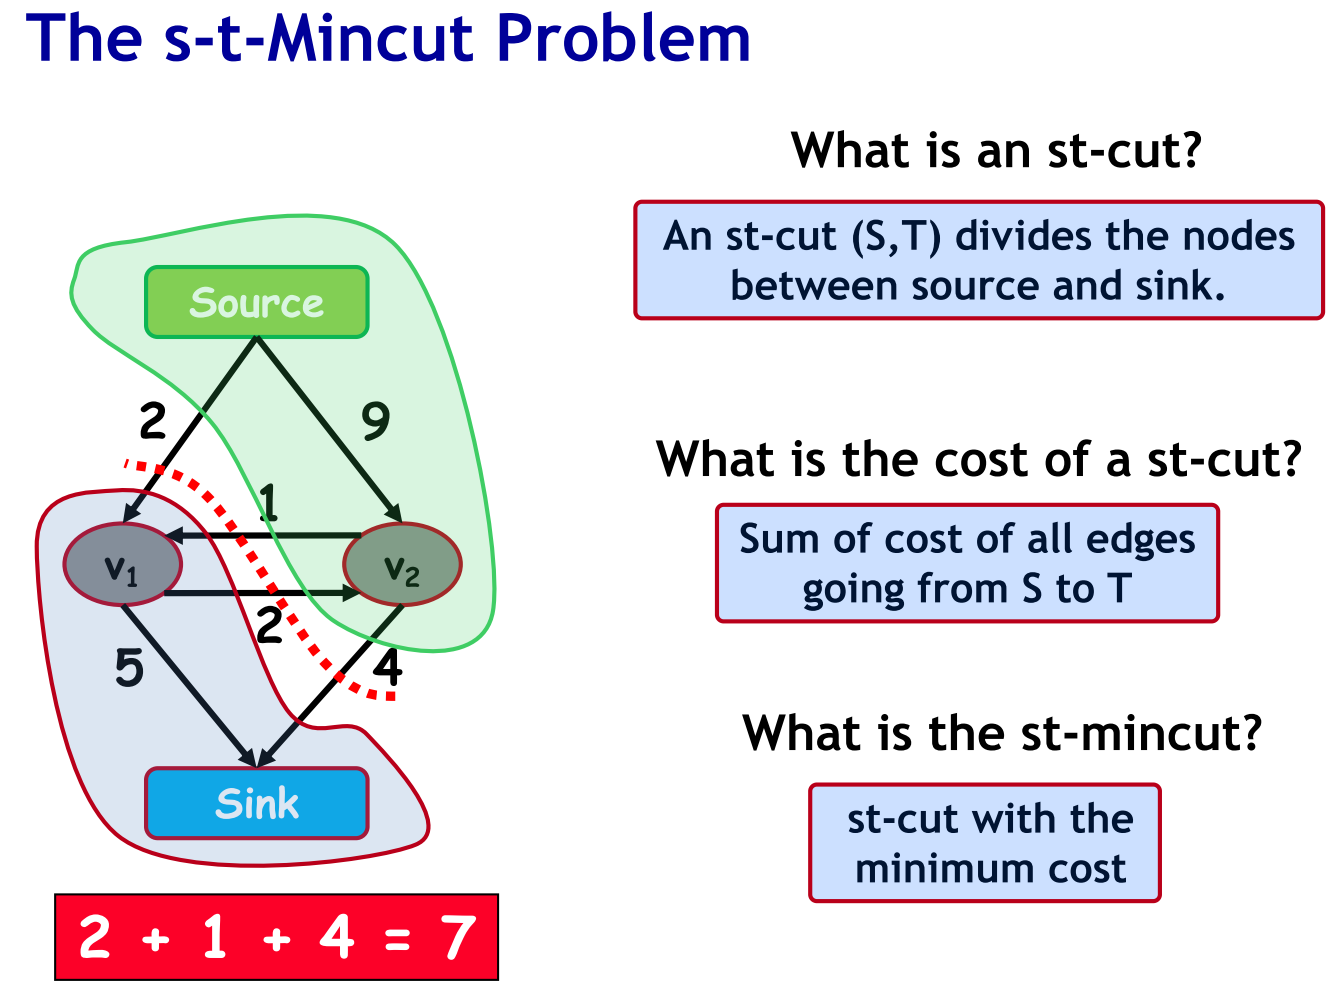
\includegraphics[width=\columnwidth]{pictures/s-t-min-cut}

Maxflow Algorithm
\begin{enumerate}
	\item Find path from source to sink with positive ! capacity
	\item push maximum possible flow through this path (subtract it from all segments)
	\item repeat until no path can be found
\end{enumerate}

Pro:
\begin{itemize}
	\item Powerful technique, based on probabilistic model (MRF).
	\item Applicable for a wide range of problems.
	\item Very efficient algorithms available for vision problems.
	\item Becoming a de-facto standard for many segmentation tasks.
\end{itemize}
Cons:
\begin{itemize}
	\item Graph cuts can solve a limited (but useful) class of models
	\item Submodular energy functions
	\item Can capture only part of the expressiveness of MRFs
	\item Only approximate algorithms available for multi-label case (except for special cases with particular topology and/or pairwise potentials)
\end{itemize}

\subsection{Learning-based approaches}
Extract the same features used during training \& Use the mapping learned before to label

\subsubsection{K-nearest neighbor}
For every point find the k nearest neighbors (labeled in the training set). The point is then defined through the lables of these neighbors (majority voting of these k neighbors)

Pro:
\begin{itemize}
	\item Very simple to implement
	\item Very simple to understand
	\item efficient implementations possible for approx. NNs
	\item distance definition is flexible
\end{itemize}
Cons:
\begin{itemize}
	\item highly depends on the definitions and k
	\item need to keep the entire data in memory for distance computations
	\item for high dimensional problems might need many training samples for accuracy
	\item other methods have better generalization ability
\end{itemize}

\subsubsection{Random forests}
Binary decision trees - Random Forests are slow to train, but fast to apply during testing.

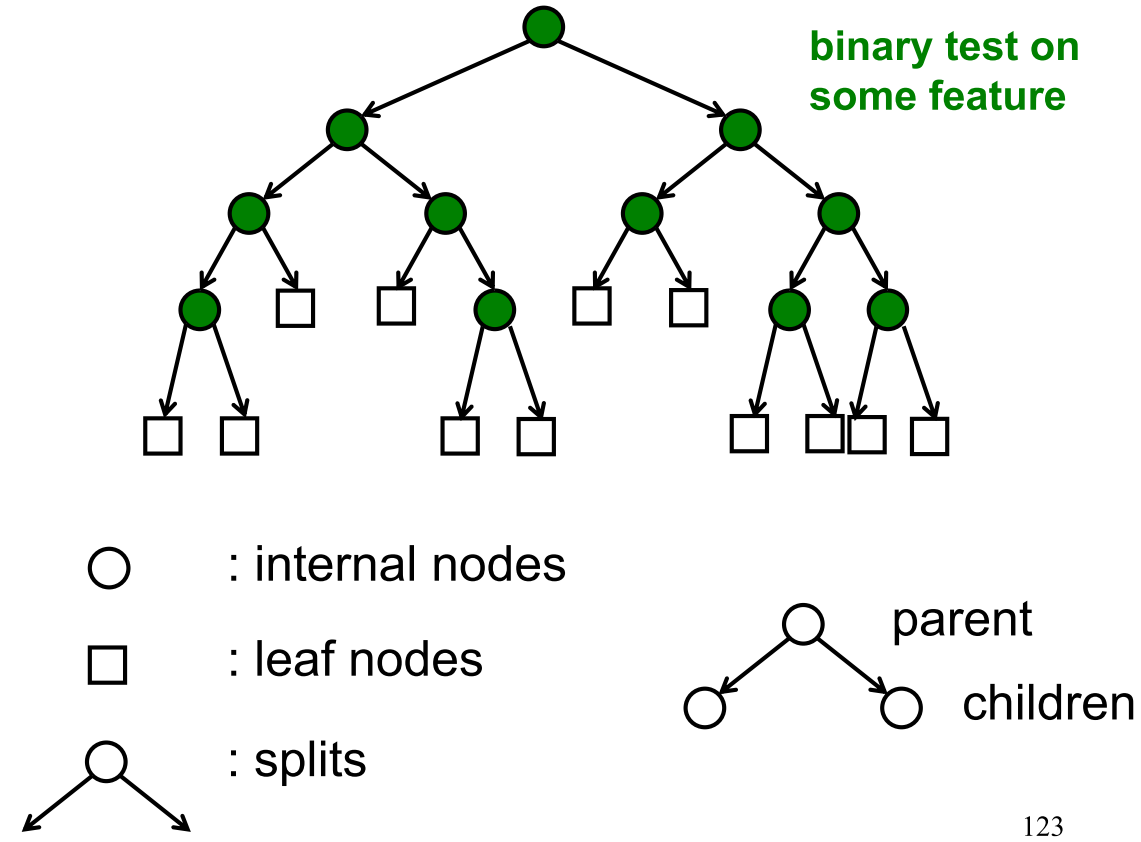
\includegraphics[width=\columnwidth]{pictures/tree}
TRaining: During training, samples are used for which the true class is known.
Having arrived at a node, one randomly generates a set of possible tests to carry out in order to split it up.
Among the possibilities one selects the test that maximally reduces the uncertainty. (biggest difference)\\
\\
Testing: Feed the current sample into every tree. See in which leaf node it ends -> (most probable) class. Combine the results, e.g. which class/label was found most often

Pro:
\begin{itemize}
	\item Easy to implement
	\item very efficient during testing
	\item can easily use diverse features
	\item can handle high dimensional spaces
\end{itemize}
Cons:
\begin{itemize}
	\item Lots of parametric choices
	\item needs large number of data
	\item training can take time
\end{itemize}		%Chapter 7 - Image Segmentation
	\section{Stereo Matching - needs work done}

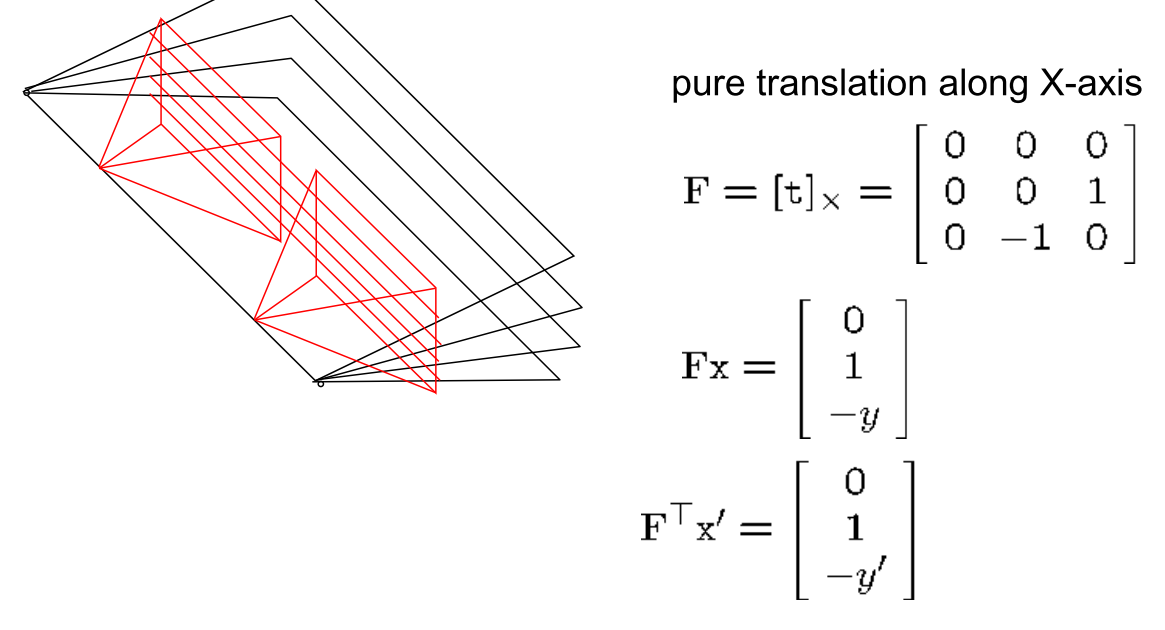
\includegraphics[width=\columnwidth]{pictures/standardstereo}


\subsection{Occlusion}
In an image pair each pixel has at most one corresponding pixel – In general one corresponding pixel – In case of occlusion there is none

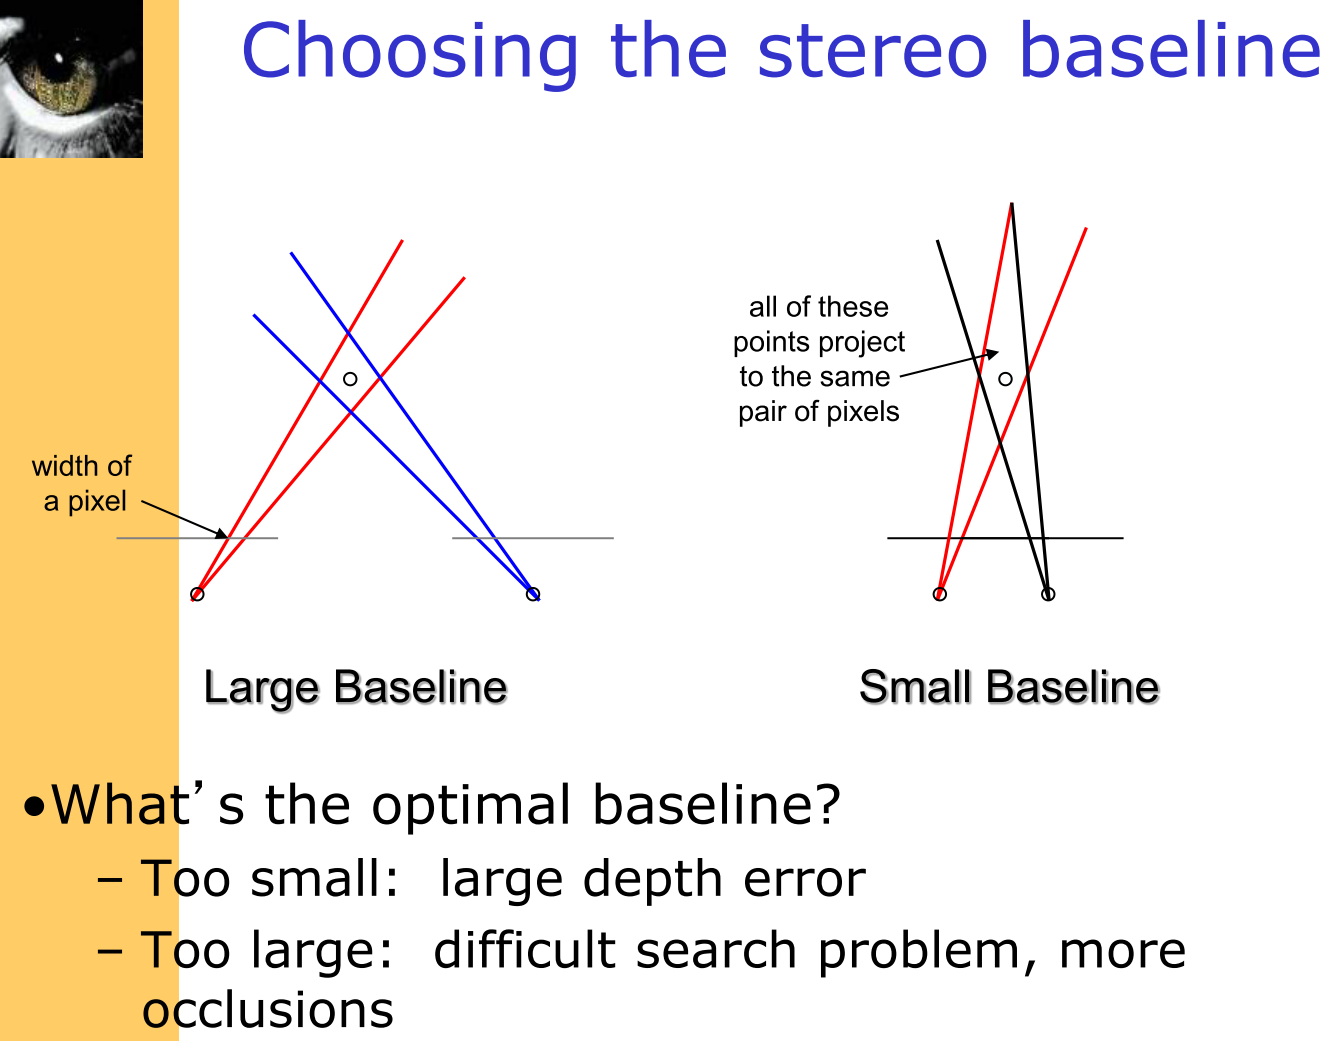
\includegraphics[width=\columnwidth]{pictures/stereobaseline}

\subsection{Deep Stereo Matching}


\subsection{3D convex hull}
The 3D convex hull of a set of 3D points is the smallest convex set which contains all 3D points.

\subsection{Visual hull}
The visual hull is the smallest volume which can be obtained by intersecting the generalized cones generated by all possible 2D shape projections ofa 3D object.\\
\\
In 3D, the visual hull is a subset ofthe convex hull. 

\subsubsection{voxel-base, marching intersections, exact polyhedral}

\subsection{Photo hull}
The photo hull is the union ofall photo-consistent volumes and the tightest possible bound on the true scene.\\
\\
It is a subset of the visual hull and - in contrast to the 3D convex hull and the visual hull depends on the texture of the 3D object.
\subsubsection{Voxel coloring}

\subsubsection{Space Carving}

Step 1: Initialize V to volume containing true scene\\
Step 2: For every voxel on surface of V test photo-consistency of voxel if voxel is inconsistent, carve it\\
Step 3: Repeat Step 2 until all voxels consistent\\
\\

Convergence: Always converges to a photo-consistent model (when all assumptions are met)
Good results on difficult real-world scenes\\
\\
Properties of Volume Intersection\\
Pros – Easy to implement, fast – Accelerated via octrees [Szeliski 1993]\\
Cons – No concavities – Reconstruction is not photo-consistent – Requires identification of silhouettes			%Chapter 8 - Stereo Matching
	\section{Structure from Motion}
\subsection{Factorization}
Factorise observations in structure of the scene and motion/calibration of the camera
Use all points in all images at the same time

\subsubsection{perspective factorization}
$$\lambda m = P M $$

\textit{something}

\subsection{structure from motion}

seriously no plan	%Chapter 9 - Structure from Motion
	\section{Specific Object Recognition}

A specific object = an instance of an object class e.g. “my car” instead of “a car”

Must overcome:
\begin{itemize}
	\item Illumination
	\item Object pose
	\item Clutter
	\item Occlusions
	\item Viewpoint
\end{itemize}

For class recognition also intra-class variation must be detected.

\subsection{Model based}
comparing image features with features of objects in a database, trying to figure out type + pose

this is SLOW and especially the need to get both object type and pose
right to formulate a correct hypothesis is problematic

\subsubsection{Invariant-based recognition of planar shapes}
The crucial advantage of invariants is that they decouple object type and pose issues

ratios of areas
are affine invariant and the following invariants are based on this

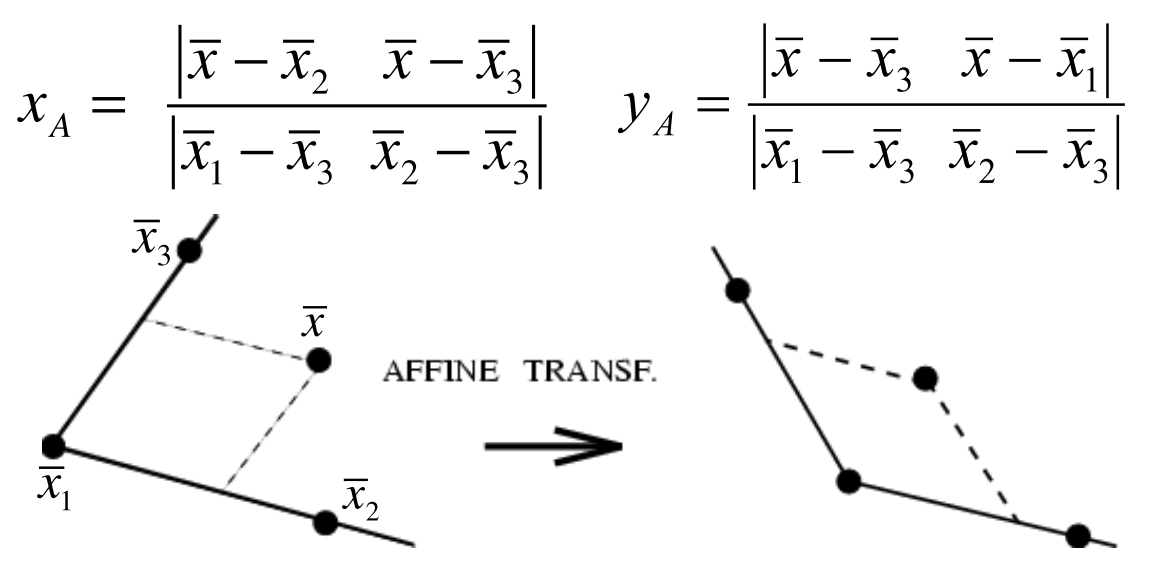
\includegraphics[width=\columnwidth]{pictures/affine}

\subsection{Image based}
PCA represents data in a lower-dimensional space keeping most of the variance
It was seen to be powerful for similar patterns like faces, that exhibit a lot of redundancy

\subsubsection{Appearance manifold approach}
Training:\\
for every object : - sample the set of viewing conditions (mainly viewpoints in this ex.)
- use these images as feature vectors (after manual bounding-box fitting around the object, rescaling, brightness normalization)
over all objects: - apply a PCA over all the images of all objects (directly on the images)
- keep the dominant PCs (10-20 enough already)
- sequence of views for 1 object represent a manifold in the space of projections (fit splines to manifolds + resample if desired)

Recognition stage (aka `Testing’)\\

Represent the incoming image as a point in the same PC space
Type: what is the nearest manifold to the point ?
Pose: what is the closest point on that closest manifold ?

\subsection{Model based vs appearance based}
Model vs Image\\

+Compact model vs -Large models
+Can deal with clutter vs -Cannot deal with clutter
-Slow analysis-by-synthesis vs +Efficient
-Models difficult to produce vs +Models easy to produce
-For limited object classes vs +For wide classes of objects

\subsection{Hybrid techniques}
\subsubsection{Euclidean invariant feature}

Training
\begin{enumerate}
	\item look for corners (with the Harris corner detector)
	\item  take circular regions around these points, of multiple radii (cope a bit with scale changes)
	\item calculate from the intensities in the circular regions . invariants under planar rotation -> feature vectors
	\item do this from different viewpoints, where the invariance cuts down on the number of views needed (here no in-plane rotations necessary)
	\item put for every object and for each of its viewpoints the . list of corner positions and their invariant feature . vectors (descriptors) in a database
\end{enumerate}

Testing
\begin{enumerate}
	\item extract corners and their invariant descriptors from the incoming image
	\item compare these invariants with those stored in the database -> find matches
	\item look for consistent placement of candidate matching corner points (e.g. using epipolar geometry)
	\item decide which object based on the number of remaining matches (i.e. consistently placed matches) (the best matching image yields the object type+appr.pose)
\end{enumerate}

\subsubsection{Recognition using local affine and photometric invariant features}
Invariant features = features that are preserved under a specific group of transformations\\



hyprid approach that aims to deal with large variations in
\begin{itemize}
	\item Viewpoint
	\item Illumination
	\item Background
	\item Occlusions
\end{itemize}





	%Chapter10 - Specific Object Recognition
	\section{Object Class Recognition}

Two main tasks: Classification and Detection

Classification: is there a car in this image ? A binary answer is enough\\
Detection: where is the car ? Need localization

\subsection{Bag of words approaches: Visual words}
\subsubsection{Local features}
Local (textured) patches (‘regions’) • Detection co-variant with translation, scale, and sometimes affine transformations
• Cover the same portion of the object in any view



Each patch / region has a descriptor, which is a point in some high-dimensional feature space (e.g., SIFT)

Close points in feature space have similar descriptors, which indicates similar image content.

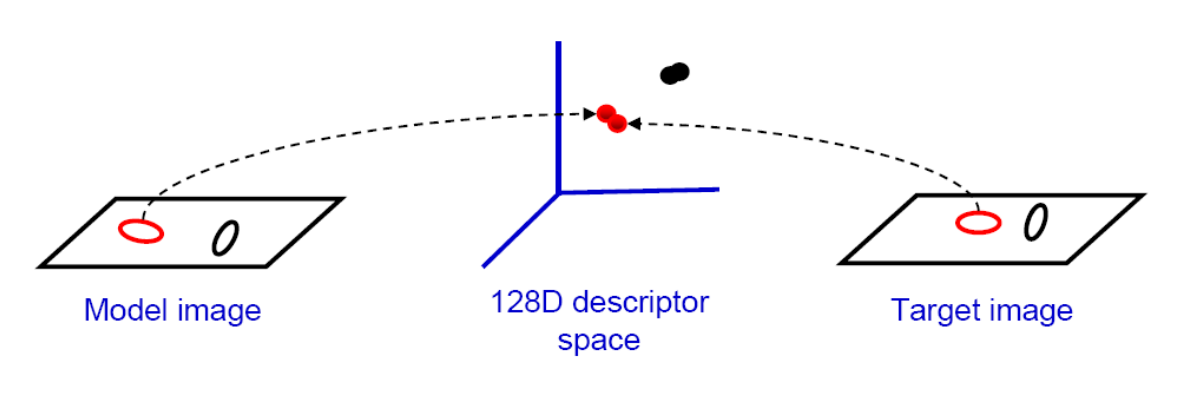
\includegraphics[width=\columnwidth]{pictures/localfeature}

\subsubsection{Visual Words}
1) Extract some local features from a number of images

2) Map high-dimensional descriptors to words by quantizing the feature space (Quantize via clustering, let cluster centers be the prototype “words”)

3) Map high-dimensional descriptors to words by quantizing the feature space. Determine which word to assign to each new image region by finding the closest cluster center

Building Visual Vocabularies
Issues: • Sampling strategy: where to extract features? ->
For object classes dense sampling works best
• Clustering / quantization algorithm ->
Many options, often k-means works well enough
• What corpus provides features (universal vocabulary?) ->
Typically as close as possible to your application • Vocabulary size, number of words\\

\subsection{Bag of Words}
Summarize entire image based on its distribution (histogram) of word occurrences.
(Analogous to bag of words representation commonly used for documents.) Quantize feature space to make discrete set of visual words

Bag of words enable to describe the unordered feature set with a single vector of fixed dimensionality

Works pretty well for whole-image classification

Classifier Choises

\begin{itemize}
	\item Nearest Neighbor
	\item Neural Networks
	\item Support Vector Machines
	\item Boosting
\end{itemize}

Nearest Neighbor - Assign label of nearest training data point to each test data point. Works very fast when training data is huge.
Support Vector Machines - Maximize the margin between the positive and negative training examples

The bag of words removes spatial layout. This is both a strength and a weakness

\subsubsection{Discussion: Bag-of-Words}
Pros:
\begin{itemize}
	\item Flexible to geometry / deformations / viewpoint
	\item Compact summary of image content
	\item Provides vector representation for sets (bags to be precise)
	\item Empirically good recognition results in practice
\end{itemize}
Cons:
\begin{itemize}
	\item Basic model ignores geometry – can verify afterwards, or embed within feature descriptors
	\item Background and foreground mixed when bag covers whole image - Interest points or sampling: no guarantee to capture object-level parts
	\item Optimal vocabulary formation remains unclear

\end{itemize}

\subsection{Classification: convolutional neural networks}
Neural network with specialized connectivity structure.

Typical building blocks of CNNs for classification in vision

\begin{itemize}
	\item Feed forward
	\item Most layers (often)
	\begin{itemize}
		\item Convolve input (filters)
		\item Non-linearity (rectified linear)
		\item Pooling (local max)
	\end{itemize}
	\item Last few layers (often)
	\begin{itemize}
		\item fully connected (linear combinations)
		\item Non-linearity (rectified linear)
	\end{itemize} 
	\item output: softmax distribution over classes
\end{itemize}
supervise, train convolutional filters by back-propagatin classification error


\subsection{Detection: Sliding-window approaches}
If object may be in a cluttered scene, slide a window around looking for it. - A brute force approach with many local decisions

\subsubsection{Gradient based Representations}
Summarize local distribution of gradients with histogram

\subsection{Boosting}
Intuition
Consider a 2D feature
space with positive and negative examples.
Each weak classifier splits the training examples with at least 50% accuracy.
Examples misclassified by a previous weak learner are given more emphasis at future rounds. Final classifier is combination of the weak classifiers

\subsection{Discussion: Sliding-Windows }
Pros
\begin{itemize}
	\item Simple detection protocol to implement
	\item Good feature choices critical
	\item Past successes for certain classes
	\item Good detectors available (Viola\&Jones, HOG, etc.)
\end{itemize}
Cons/Limitations
\begin{itemize}
	\item High computational complexity 
	\begin{itemize}
		\item – For example: 250,000 locations x 30 orientations x 4 scales = 30,000,000 evaluations!
		\item This puts tight constraints on the classifiers we can use.
		\item If training binary detectors independently, this means cost increases linearly with number of classes.
	\end{itemize}
	\item With so many windows, false positive rate better be low
	\item Typically need fully supervised training data (= bounding-boxes)
	\item Some object do not fit a box well (diagonal bottle) Sensitive to partial occlusion (unless in training data)
\end{itemize}

\subsection{Detection: proposal-based approaches}
\subsubsection{Object proposals}
Every object has at least one of these properties
• Well-defined, closed boundary in space • Different appearance than its surroundings • Might be unique within the image (salient)

Objectness(w) = probability that w covers an object

Objectness cues
\begin{itemize}
	\item Density of salient pixels
	\item color contrast
	\item superpixel straddling
\end{itemize}
\subsubsection{R-CNN}
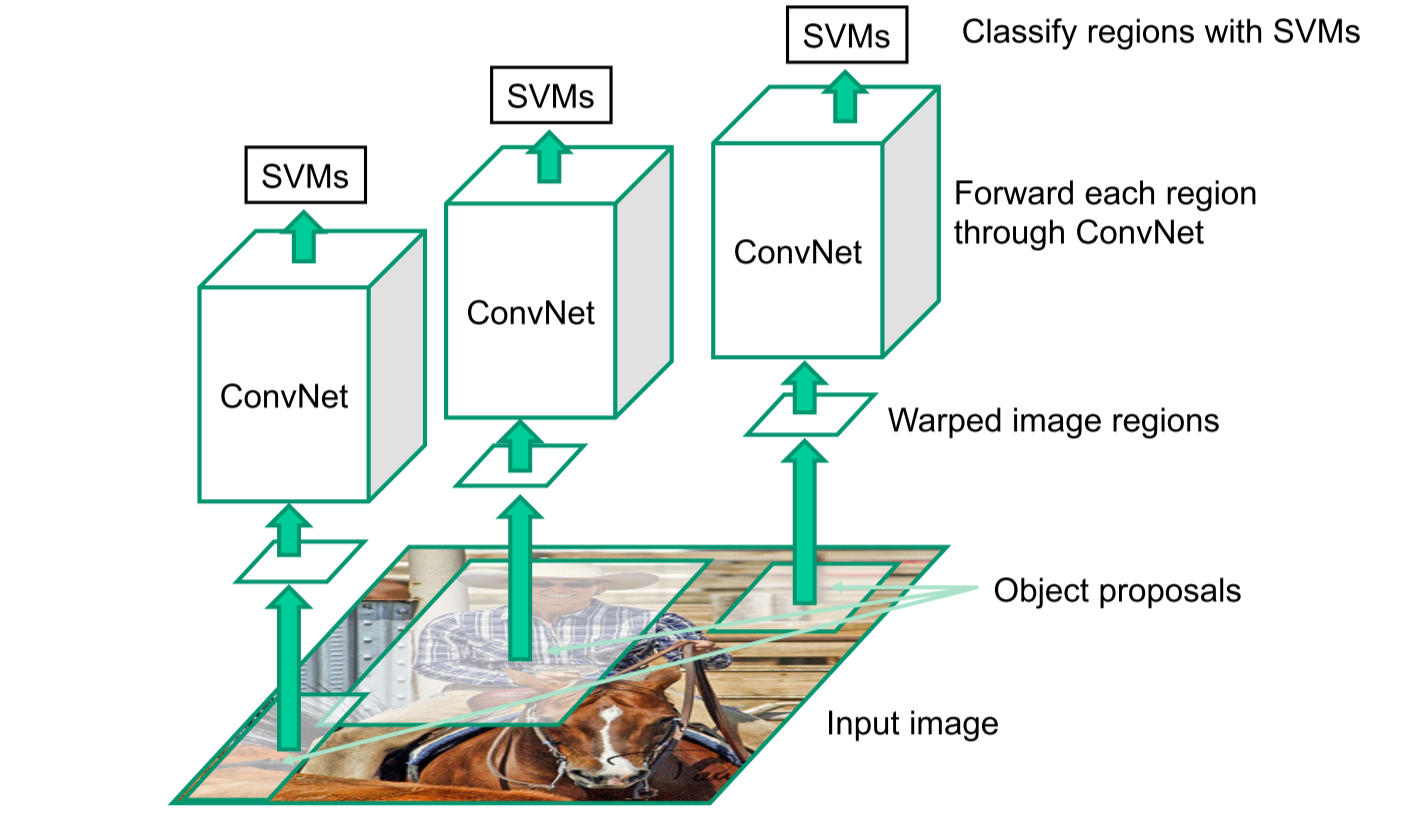
\includegraphics[width=\columnwidth]{pictures/R-CNN}
Pros
\begin{itemize}
	\item Accurate!
	\item Any deep architecture can immediately be plugged in
\end{itemize}
Cons
\begin{itemize}
	\item Ad hoc training objectives
	\begin{itemize}
		\item Fine-tuning network with softmax classifier (log loss)
		\item Train post-hoc linear SVMs (hinge loss)
		\item Train post-hoc bounding-box regressions (least squares)
	\end{itemize}
	\item Training is slow (84h), takes a lot of disk space
	\item Inference (detection) is slow
\end{itemize}
\subsubsection{Fast R-CNN}
Full Image first through ConvNet and afterwards Region selection
\subsection{Detection: a star model}
Recognition of object categories

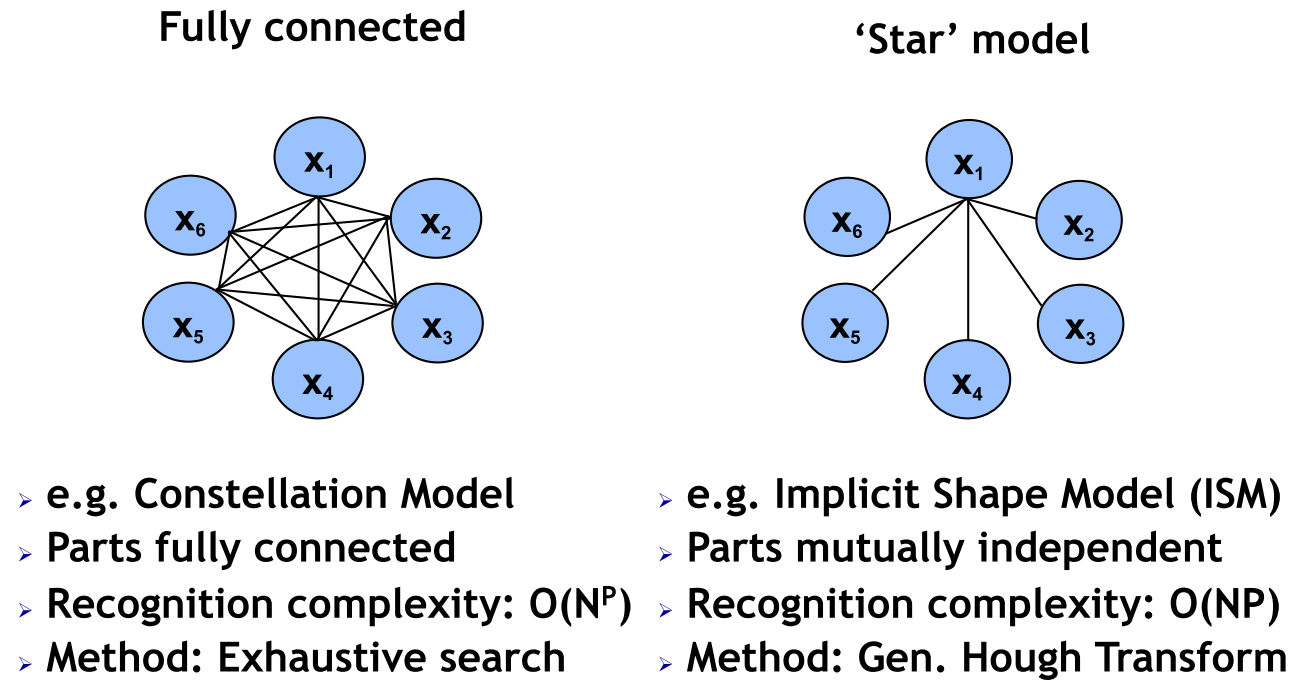
\includegraphics[width=\columnwidth]{pictures/star_models}

\subsubsection{Implicit Shape Model}
Visual vocabulary is used to index votes for object position [a visual word = a “part”].
Objects are detected as consistent configurations of the observed parts (visual words).

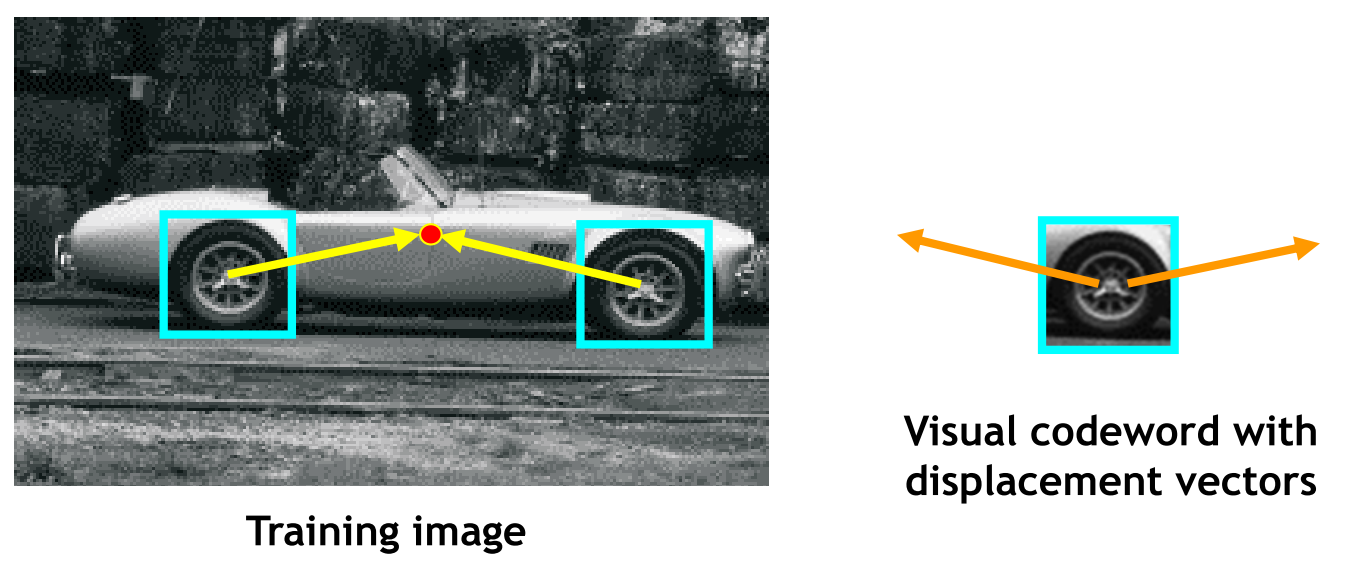
\includegraphics[width=\columnwidth]{pictures/ISM}
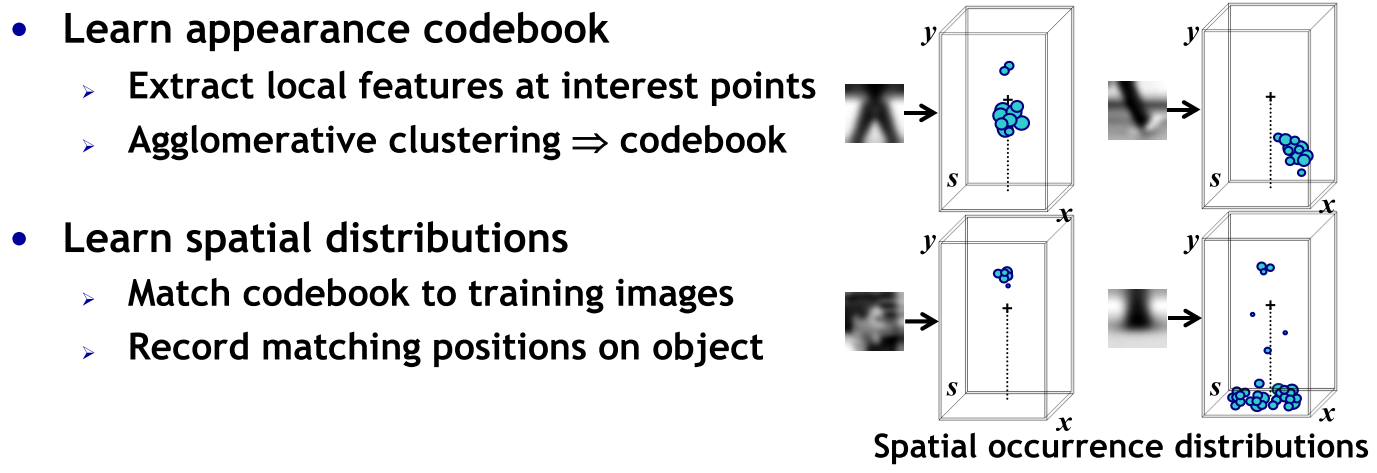
\includegraphics[width=\columnwidth]{pictures/ism_spatial}


Pros:
\begin{itemize}
	\item Works well for many different object categories – Both rigid and articulated objects
	\item Flexible geometric model – Can recombine parts seen on different training examples
	\item Learning from relatively few (50-100) training examples
	\item Optimized for detection, good localization properties
\end{itemize}
Cons:
\begin{itemize}
	\item Needs supervised training data – Object bounding boxes for detection \& Segmentations for top-down segmentation
	\item Only weak geometric constraints – Result segmentations may contain superfluous body parts.
	\item Purely representative model – No discriminative learning
\end{itemize}
%Chapter11 - Object Class Recognition
	
	
\end{multicols*}
\begin{multicols*}{3}	
	\appendix
	\section{Glossary}
\paragraph{Mode} = local maximum of a given distribution
\paragraph{k-means vs knn}   KNN represents a supervised classification algorithm that will give new data points accordingly to the k number or the closest data points,
while k-means clustering is an unsupervised clustering algorithm that gathers and groups data into k number of clusters.				%A Glossary
	

	
	
\end{multicols*}
\end{document}